% ---------- Titelblad Masterproef Faculteit Wetenschappen -----------
% Dit document is opgesteld voor compilatie met pdflatex.  Indien je
% wilt compileren met latex naar dvi/ps, dien je de figuren naar
% (e)ps-formaat om te zetten.
%                           -- december 2012
% -------------------------------------------------------------------
\RequirePackage{fix-cm}
\documentclass[12pt,a4paper,oneside]{book}

% --------------------- In te laden pakketten -----------------------
% Deze kan je eventueel toevoegen aan de pakketten die je al inlaadt
% als je dit titelblad integreert met de rest van thesis.
% -------------------------------------------------------------------
\usepackage[dutch]{babel}
\usepackage{graphicx,xcolor,textpos}
\usepackage[utf8]{inputenc}
\usepackage[T1]{fontenc}
\usepackage{helvet}
\usepackage{amsmath}
\usepackage{listings}
\usepackage{hyperref}
\usepackage[hypcap]{caption}
\usepackage{color}
\usepackage{longtable}
\usepackage{booktabs}
\usepackage{pgfplotstable}
\usepackage{needspace}
\usepackage[toc,page]{appendix}
\usepackage{ltablex}

% -------------------- Pagina-instellingen --------------------------
% Indien je deze wijzigt, zal het titelblad ook wijzigen.  Dit dien je
% dan manueel aan te passen.
% --------------------------------------------------------------------
\topmargin -10mm
\textwidth 160truemm
\textheight 240truemm
\oddsidemargin 0mm
\evensidemargin 0mm

% ------------------- textpos-instellingen ---------------------------
% Enkele andere instellingen voor het voorblad.
% --------------------------------------------------------------------
\definecolor{green}{RGB}{172,196,0}
\definecolor{bluetitle}{RGB}{29,141,176}
\definecolor{blueaff}{RGB}{0,0,128}
\definecolor{blueline}{RGB}{82,189,236}
\definecolor{dkgreen}{rgb}{0,0.6,0}
\definecolor{gray}{rgb}{0.5,0.5,0.5}
\definecolor{mauve}{rgb}{0.58,0,0.82}
\setlength{\TPHorizModule}{1mm}
\setlength{\TPVertModule}{1mm}

% Eigen instellingen
%\setdefaultlanguage{dutch}
\newcommand{\powerTable}[3]{
    \Needspace{15\baselineskip}
    \pgfplotstabletypeset[
        string type,
        col sep = comma,
        skip rows between index={0}{#2},
        skip rows between index={#3}{1000000000},
        begin table=\begin{longtable},
        end table=\end{longtable},
        % packo id,N,Packomania Radius,,id,circlecount,Radius,time (ns),overlap (square units),nancount,Time,,Difference,% Increase
        columns={{N},{ratio},{Radius},{Difference},{Increase},{Time}},
        every head row/.style={before row=\caption[]{#1}\\\toprule, after row=\midrule\endhead},
        every last row/.style={after row=\bottomrule},
        every first row/.style={before row=\captionsetup{labelformat=empty}\caption[#1]{}\\[-23pt]},
        column type={l}, %default
        columns/{N}/.style={column type={c}},
        columns/{ratio}/.style={column name={Beste radius}},
        columns/{Radius}/.style={column name={Radius}},
        columns/{Difference}/.style={column name={Vergroting}},
        columns/{Increase}/.style={column type={c}, column name={Vergroting (\%)}},
        columns/{Time}/.style={column name={Tijd}},
    ]{csv/Power Packomania Problems Comparison.csv}
}





\newcommand{\equalTable}[3]{
    \Needspace{15\baselineskip}
    \pgfplotstabletypeset[
        string type,
        col sep = comma,
        skip rows between index={0}{#2},
        skip rows between index={#3}{1000000000},
        begin table=\begin{longtable},
        end table=\end{longtable},
        % N,radius,distance,ratio,density,contacts,loose,boundary,symmetry group,reference,,id,circlecount,Radius,time (ns),overlap (square units),nancount,Time,,Difference,Increase
        columns={{N},{ratio},{Radius},{Difference},{Increase},{Time}},
        every head row/.style={before row=\caption[]{#1}\\\toprule, after row=\midrule\endhead},
        every last row/.style={after row=\bottomrule},
        every first row/.style={before row=\captionsetup{labelformat=empty}\caption[#1]{}\\[-23pt]},
        column type={l}, %default
        columns/{N}/.style={column type={c}},
        columns/{ratio}/.style={column name={Beste radius}},
        columns/{Radius}/.style={column name={Radius}},
        columns/{Difference}/.style={column name={Vergroting}},
        columns/{Increase}/.style={column type={c}, column name={Vergroting (\%)}},
        columns/{Time}/.style={column name={Tijd}},
    ]{csv/Equal size Packomania problems comparison.csv}
}





\newcommand{\benchmarkTable}[3]{
    \Needspace{15\baselineskip}
    \pgfplotstabletypeset[
        string type,
        col sep = comma,
        skip rows between index={0}{#2},
        skip rows between index={#3}{1000000000},
        begin table=\begin{longtable},
        end table=\end{longtable},
        % instance,N,radius,ratio,density,,id,circlecount,Radius,time (ns),overlap (square units),nancount,Time,,Difference,Increase
        columns={{instance},{N},{ratio},{Radius},{Difference},{Increase},{Time}},
        every head row/.style={before row=\caption[]{#1}\\\toprule, after row=\midrule\endhead},
        every last row/.style={after row=\bottomrule},
        every first row/.style={before row=\captionsetup{labelformat=empty}\caption[#1]{}\\[-23pt]},
        column type={l}, %default
        columns/{instance}/.style={column name={Instantie}},
        columns/{N}/.style={column type={c}},
        columns/{ratio}/.style={column name={Beste radius}},
        columns/{Radius}/.style={column name={Radius}},
        columns/{Difference}/.style={column name={Vergroting}},
        columns/{Increase}/.style={column type={c}, column name={Vergroting (\%)}},
        columns/{Time}/.style={column name={Tijd}},
    ]{csv/IN NR Packomania problems comparison.csv}
}

\graphicspath{{images/}}
\renewcommand{\contentsname}{Inhoud}
\renewcommand{\listfigurename}{Lijst van figuren}
\renewcommand{\listtablename}{Lijst van tabellen}
\renewcommand{\chaptername}{Hoofdstuk}
\renewcommand{\chapterautorefname}{hoofdstuk}
\renewcommand{\sectionautorefname}{sectie}
\renewcommand{\subsectionautorefname}{sectie}
\renewcommand{\figureautorefname}{figuur}
\renewcommand{\tableautorefname}{tabel}
\newcommand{\lstnumberautorefname}{lijn}
\renewcommand{\appendixautorefname}{bijlage}

\lstset{frame=tb,
  language=Java,
  aboveskip=3mm,
  belowskip=3mm,
  showstringspaces=false,
  columns=flexible,
  basicstyle={\small\ttfamily},
  numbers=left,
  numberstyle=\tiny\color{gray},
  keywordstyle=\color{blue},
  commentstyle=\color{dkgreen},
  stringstyle=\color{mauve},
  breaklines=true,
  breakatwhitespace=true,
  tabsize=4,
  escapechar=|
}

% begin appendix autoref patch [\autoref subsections in appendix](http://tex.stackexchange.com/questions/149807/autoref-subsections-in-appendix)
\usepackage{etoolbox}
\makeatletter
\patchcmd{\hyper@makecurrent}{%
    \ifx\Hy@param\Hy@chapterstring
        \let\Hy@param\Hy@chapapp
    \fi
}{%
    \iftoggle{inappendix}{%true-branch
        % list the names of all sectioning counters here
        \@checkappendixparam{chapter}%
        \@checkappendixparam{section}%
        \@checkappendixparam{subsection}%
        \@checkappendixparam{subsubsection}%
        \@checkappendixparam{paragraph}%
        \@checkappendixparam{subparagraph}%
    }{}%
}{}{\errmessage{failed to patch}}

\newcommand*{\@checkappendixparam}[1]{%
    \def\@checkappendixparamtmp{#1}%
    \ifx\Hy@param\@checkappendixparamtmp
        \let\Hy@param\Hy@appendixstring
    \fi
}
\makeatletter

\newtoggle{inappendix}
\togglefalse{inappendix}

\apptocmd{\appendix}{\toggletrue{inappendix}}{}{\errmessage{failed to patch}}
\apptocmd{\subappendices}{\toggletrue{inappendix}}{}{\errmessage{failed to patch}}
% end appendix autoref patch

\begin{document}

% ---------------------- Voorblad ------------------------------------
% Vergeet niet de tekst aan te passen:
% - Titel en, indien van toepassing, ondertitel
%          voor eventuele formules in de titel of ondertitel
%          gebruik je  \form{$...$}
% - Je naam
% - Je (co)promotor, begeleider (indien van toepassing)
% - Je opleiding
% - Het academiejaar
% --------------------------------------------------------------------
\thispagestyle{empty}
\newcommand{\form}[1]{\scalebox{1.087}{\boldmath{#1}}}
\sffamily
%
\begin{textblock}{191}(-24,-11)
\colorbox{green}{\hspace{123mm}\ \parbox[c][18truemm]{68mm}{\textcolor{white}{FACULTEIT WETENSCHAPPEN}}}
\end{textblock}
%
\begin{textblock}{70}(-18,-19)
\textblockcolour{}
\includegraphics*[height=19.8truemm]{LogoKULeuven.png}
\end{textblock}
%
\begin{textblock}{79}(50,50)
\centerline{\includegraphics*[height=10.0truecm]{voorbladpacking.png}}
%De achtergrond kan wit blijven of je kan een afbeelding invoegen (maximum hoogte 10 cm, breedte variabel, denk aan auteursrechten\ldots). GEEN logo's (je kan binnenin de masterproef logo's gebruiken, maar niet op de voor- of achterpagina).
\end{textblock}
%
\begin{textblock}{160}(-6,63)
\textblockcolour{}
\vspace{-\parskip}
\flushleft
\fontsize{40}{42}\selectfont \textcolor{bluetitle}{Een nieuwe constructieve heuristic voor het plaatsen van cirkels in een cirkel}\\[1.5mm]
\fontsize{20}{22}\selectfont Gebaseerd op een \textit{best-fit} methodiek
\end{textblock}
%
\begin{textblock}{160}(8,153)
\textblockcolour{}
\vspace{-\parskip}
\flushright
\fontsize{14}{16}\selectfont \textbf{Pablo BOLLANSÉE}
\end{textblock}
%
\begin{textblock}{70}(-6,191)
\textblockcolour{}
\vspace{-\parskip}
\flushleft
Promotor: Prof. P. De Causmaecker \\[-2pt]
\textcolor{blueaff}{Affiliatie \textsl{(facultatief)}}\\[5pt]
Co-promotor: \textsl{(facultatief)}\\[-2pt]
\textcolor{blueaff}{Affiliatie \textsl{(facultatief)}}\\[5pt]
Begeleider: \textsl{(facultatief)}\\[-2pt]
\textcolor{blueaff}{Affiliatie \textsl{(facultatief)}}\\
\end{textblock}
%
\begin{textblock}{160}(8,191)
\textblockcolour{}
\vspace{-\parskip}
\flushright
Proefschrift ingediend tot het\\[4.5pt]
behalen van de graad van\\[4.5pt]
Master of Science in de\\[4.5pt]
toegepaste informatica\\
\end{textblock}
%
\begin{textblock}{160}(8,232)
\textblockcolour{}
\vspace{-\parskip}
\flushright
Academiejaar 2015-2016
\end{textblock}
%
\begin{textblock}{191}(-24,248)
{\color{blueline}\rule{550pt}{5.5pt}}
\end{textblock}
%
\vfill

\newpage
\thispagestyle{empty}
\begin{textblock}{160}(0,185)
© Copyright by KU Leuven

Zonder voorafgaande schriftelijke toestemming van zowel de promotor(en) als de auteur(s) is overnemen, kopiëren, gebruiken of realiseren van deze uitgave of gedeelten ervan verboden. Voor aanvragen tot of informatie i.v.m. het overnemen en/of gebruik en/of realisatie van gedeelten uit deze publicatie, wendt u tot de KU Leuven, Faculteit Wetenschappen, Geel Huis, Kasteelpark Arenberg 11 bus 2100, 3001 Leuven (Heverlee), Telefoon +32 16 32 14 01.

Voorafgaande schriftelijke toestemming van de promotor(en) is eveneens vereist voor het aanwenden van de in dit afstudeerwerk beschreven (originele) methoden, producten, schakelingen en programma’s voor industrieel of commercieel nut en voor de inzending van deze publicatie ter deelname aan wetenschappelijke prijzen of wedstrijden.
\end{textblock}

\newpage

% Als je het titelblad wil integreren met de rest van je thesis,
% kan je hieronder verder.
% ----------------------- Eerste pagina's -------------------------
% Hier kan je inhoudsopgave, voorwoord en dergelijke kwijt.
% -----------------------------------------------------------------
\rmfamily
\setcounter{page}{0}
\pagenumbering{roman}

\newpage

\chapter*{Voorwoord}
\addcontentsline{toc}{chapter}{Voorwoord}

Het circle-packing probleem bestaat er uit om een aantal cirkels, met gekende radii, in een zo klein mogelijke container te plaatsen.
De vorm van deze container kan verschillen, meestal is het een driehoek, rechthoek of cirkel.
In deze thesis stel ik een nieuwe \textit{best-fit} gebaseerde heuristiek voor voor het plaatsen van cirkels in een cirkel.
Het is een constructieve heuristiek waarin stapsgewijs telkens de best-passende cirkel geplaatst zal worden.
Alle code is beschikbaar op GitHub \cite{circle-packing-github}

Wiskundig is dit een relatief eenvoudig probleem om voor te stellen, maar computationeel is het zeer zwaar om exact op te lossen.
Bestaande pogingen om dit probleem op te lossen vragen zeer veel tijd om het te berekenen.
In deze thesis stel ik een nieuwe heuristiek voor die het mogelijk maakt zéér snel oplossingen te genereren.

Ik wil hierbij Patrick De Causmaeker bedanken voor alle hulp en ondersteuning bij het ontwerpen van deze heuristiek en verwezenlijken van dit werk.
Ook wil ik Jim Bollansée, Marie Julia Bollansée en Pieter Van de Walle bedanken voor hun hulp bij het schrijven van deze tekst.

%  In het voorwoord wordt de algemene doelstelling van het werk samengevat
%  in enkele regels en worden personen, diensten of firma’s bedankt voor hun
%  medewerking bij het tot stand komen van het werk.
%  De naam van firma’s en personen uit deze firma’s mogen slechts worden vermeld
%  mits hun uitdrukkelijke toelating én na overleg met de supervisor(en)! Steeds
%  wordt de supervisor(en) vermeld, de verantwoordelijke en eventueel de personen
%  die rechtstreeks geholpen hebben bv. door het ter beschikking stelling van
%  meetresultaten, faciliteiten. Ook de instantie die eventueel een doctoraatsbeurs
%  heeft toegekend wordt bedankt (bv. FWO, IWT, . . . ).

\newpage

\chapter*{Abstract}
\addcontentsline{toc}{chapter}{Abstract}

TODO

%  In een beknopte tekst van maximum 2 pagina’s worden de belangrijkste
%  doelstellingen en besluiten geformuleerd, zowel in het Nederlands als in het
%  Engels. Zulke samenvattingen kunnen worden gebruikt in wetenschappelijke
%  verslagen van het departement of de faculteit. Het Engels moet vlekkeloos zijn.

\newpage

\tableofcontents
\listoffigures
\addcontentsline{toc}{chapter}{Lijst van figuren}
\listoftables
\addcontentsline{toc}{chapter}{Lijst van tabellen}

\newpage

% ----------------------- Eigenlijke thesis -----------------------
% Vanaf de inleiding/het eerste hoofdstuk.
% -----------------------------------------------------------------
\setcounter{page}{0}
\pagenumbering{arabic}

\chapter{Inleiding}

In deze thesis stel ik een nieuwe \textit{best-fit} gebaseerde heuristiek voor om het \textit{circle-packing} probleem.
De heuristiek is specifiek ontworpen voor het sub-probleem van het plaatsen van cirkels in een cirkel.
Het \textit{circle-packing} probleem bestaat uit het plaatsen van $n$ cirkels in een zo klein mogelijke cirkelvormige \textit{container}.
Het is de bedoeling om voor de gegeven cirkels de coordinaten van de middelpunten te vinden zodat de cirkels niet overlappen en de radius van de omcirkel zo klein mogelijk is.

Circle-packing is zowel theoretisch als praktisch een zeer interessant probleem.
Het kan gebruikt worden om verschillende \textit{real-world} problemen op te lossen, zoals het plaatsen van zendmasten, stokage van cilindrische voorwerpen, en het combineren van verschillende kabels. //TODO voeg referenties toe voor deze gebruiken

Mathematisch is het probleem redelijk eenvoudig als een optimalisatieprobleem te omschrijven:

\begin{equation*}
\begin{aligned}
& \text{minimaliseer}
& & r \\
& \text{onderhevig aan}
& & x_i^2 + y_i^2 \leq (r-r_i)^2, 
& & &i = {1,...,n}\\
&&& (x_i - x_j)^2 + (y_i - y_j)^2 \geq (r_i + r_j)^2,
& & &i \neq j
\end{aligned}
\end{equation*}

Hierin is $r_i$ de radius, en $(x_i,y_i)$ de coördinaten van het centrum van cirkel $i$.
Hierbij wordt verondersteld dat de omcirkel het nulpunt als middelpunt heeft.
De eerste formule verzekert dat de cirkels in de omcirkel liggen, en de tweede dat ze elkaar niet overlappen.
Wanneer alle cirkels dezelfde grootte hebben, wordt meestal $r_i$ gelijk aan $1$ genomen.
Het circle-packing probleem voor andere containers heeft gelijkaardige, relatief eenvoudige, wiskundige omschrijvingen.

Hoewel dit wiskundig eenvoudig te omschrijven is, blijft het toch een zeer moeilijk probleem om exact op te lossen.
Er is reeds veel onderzoek gebeurd naar het oplossen van het circle-packing probleem voor zowel cirkels van gelijke gootte, als voor cirkels van verschillende grootte.
In \cite{graham1996repeated} en \cite{lubachevsky1997curved} probeert men vaste patronen te vinden die een optimale packing van cirkels met gelijke grootte geeft.
In \cite{graham1998dense} en \cite{wang2002improved} worden fysisch geïnspireerde simulaties gebruikt om packing te bekomen.
In \cite{george1995packing} worden verschillende meta-heuristieken, waaronder een genetisch algoritme, uitgeprobeerd en vergeleken.
Zij ondervinden dat dit genetisch algoritme, als ook een quasi-random techniek, in vergelijking met de andere uitgeprobeerde meta-heuristieken, de beste resultaten geven.
In \cite{hifi2004approximate} en \cite{hifi2004simulated} worden respectievelijk een genetisch en een simulated-annealing algoritme voorgesteld.
Een recentere poging is het Monotonic Basin Hopping algoritme voorgesteld in \cite{grosso2010}.
Hierin beschrijven de auteurs dat er te veel lokale optima zijn voor een eenvoudige multi-start behandeling, en stellen een variant voor waarin ze op een slimme manier de begin punten proberen genereren.
Ook meer recent zijn \cite{jors2011} (2011), \cite{ye2013iterated} (2013) en \cite{zeng2016iterated} (2016).
Hierin worden de combinatorische eigenschappen van circle-packing in combinatie met een zoekmethode zoals \textit{tabu-search} en \textit{iterated local search} gebruikt om een goede volgorde te vinden waarin de cirkels geplaatst worden.
In \cite{jors2011} plaatsen ze zo één voor één elke cirkel en berekend een \textit{non-linear optimizer} hiervoor telkens een lokaal extremum voor de \textit{packing}.

Constructieve algoritmen voor het oplossen van circle-packings zijn veel minder onderzocht.
Een constructief algoritme is een algoritme dat, beginnende van een zekere begin situatie, stapsgewijs de oplossing uitbreidt tot een volledige oplossing bekomen is.
Eén van de weinige constructieve methoden wordt beschreven in \cite{akeb2006basic}, waar ze een alternatieve vorm van het \textit{circle-packing} probleem oplossen: de grootte van de container ligt vast, en er moeten zo veel mogelijk cirkels van gelijke grootte in de container geplaatst worden.
In \cite{hifi2004approximate} wordt er een aanpassing gedaan op de klassieke bottom-left-first heuristiek, voor het plaatsen van rechthoeken.
Deze heuristiek plaats rechthoeken zo ver mogelijk in de linker beneden hoek.
Dit is een zeer eenvoudige heuristiek die redelijk goede resultaten geeft.
Zij hebben deze dan aangepast om cirkels in een rechthoek te plaatsen.

Hoewel veel van deze oplossingen zeer goede packings maken, en regelmatig hun voorgangers verbeteren, vragen ze veel rekentijd en beperken ze zich tot een klein aantal cirkels.
Voor slechts tientallen cirkels kan de nodige rekentijd oplopen tot tientallen uren.
In deze thesis stel ik een nieuw constructieve heuristiek voor om het circle-packing probleem op te lossen.
Deze nieuwe heuristiek laat toe om packings te maken in een fractie van de tijd die andere algoritmen daarvoor nodig hebben.
Ook is het mogelijk om veel grotere aantallen cirkels te plaatsen.
De omcirkel van packings verkregen met deze nieuwe heuristiek is echter iets groter dan deze verkregen in voorgenoemd onderzoek.
Deze uitbreiding van de omcirkel blijft echter beperkt en laat toe de packings in slecht enkele ogenblikken te maken, waar anderen uren rekentijd vragen.

De heuristiek voorgesteld in deze thesis is een best-fit heuristiek gebaseerd op een oplossing voor het Orthogonal Stock-Cutting Problem voorgesteld in \cite{burke2004new}.
In dit probleem worden balken geplaatst in een container met een vaste breedte, zodat de hoogte zo klein mogelijk blijft.
Zij gebruiken het verschil tussen de breedte van een balk en een gat in de packing als heuristiek voor de \textit{beste} positie.
Hun heuristiek kiest dus de volgende balk om te plaatsen uit een lijst, en deze plaatst op de \textit{beste} positie.
Dit is in tegenstelling tot cirkels plaatsen in een vooraf bepaalde volgorde zoals in \cite{grosso2010} en \cite{jors2011}.
Op een gelijkaardige manier kiest mijn algoritme de volgende cirkel die best past in de huidige packing.

In \autoref{chap:algoritme} bespreek ik hoe de heuristiek opgebouwd is.
Ik beschrijf de twee basisconcepten voor mijn best-fit heuristiek, \textit{holes} en de \textit{shell}, in detail.
Ik bespreek hoe deze werken, en op welke manier gekozen wordt welke cirkel best past in de packing.
Hierbij haal ik ook de implementatie aan om deze concepten te verduidelijken.
In \autoref{chap:resultaten} worden de verkregen resultaten besproken.
Hier vergelijk ik de packings met de best gekende resultaten zoals gerapporteerd op de Packomania website (\cite{packomania}).
De Packomania website verzameld alle best gekende oplossingen voor verschillende circle-packing problemen.
Ik vergelijk de omtrek van de verkregen omcirkel en de nodige tijd om de packing te berekenen van mijn eigen heuristiek met de best gekende oplossingen op de Packomania website.
Ook toon ik resultaten voor packings voor veel meer cirkels dan getoond op de Packomania website.
In \autoref{chap:bedenkingen} bespreek ik enkele bedenkingen die ik heb bij de heuristiek en zijn implementatie.
In \autoref{chap:verder-werk} bespreek ik mogelijke verbeteringen en ideeën voor verder onderzoek.
In \autoref{chap:handleiding-visualisaties} wordt kort verduidelijkt hoe de visualisaties te interpreteren die doorheen deze thesis gebruikt worden.
Maar eerst worden enkele termen die gebruikt worden in de verdere tekst, sommige uniek voor voor deze heuristiek, en definities gegeven in \autoref{chap:definities}.

// TODO: Is het nodig sommige termen te verduidelijken? De termen: NP-Moeilijk, meta-heuristiek, genetisch algoritme, quasi-random techniek, simulated-annealing, tabu-search, bottom-left-first heuristiek -> Ja. TODO
% TODO: Vraag voor Patrick: Is het nodig de aangehaalde papers verder te verduidelijk? Of zijn de zeer korte besprekingen zoals ze nu zijn genoeg? -> Korte zijn genoeg

\chapter{Definities en termen} \label{chap:definities}

\textbf{Cirkel} In de literatuur rond \textit{circle-packing} en deze thesis wordt het woord "cirkel" of "circle" gebruikt, maar eigenlijk zou het correcter zijn om "schijf" te gebruiken.
Er is dus ook een overlap tussen cirkels wanneer een cirkel volledig omringd is door een andere.
Voor twee cirkels met radii $r_a, r_b$ en coordinaten  $(x_a,y_a), (x_b,y_b)$ is er een overlap wanneer $r_a + r_b > \sqrt{(x_a-x_b)^2 + (y_a-y_b)^2}$. 

\textbf{Packing} of \textbf{Plaatsing} Is een collectie cirkels met elks een toegewezen positie. Een packing is correct wanneer er geen overlap is tussen de cirkels in de packing.

\textbf{Holes} Is één van de concepten uniek aan deze heuristiek. Op een \textit{high-level} niveau is dit een plek tussen drie cirkels waar nog een andere cirkel kan geplaatst worden. Dit wordt in diep detail uitgelegd in \autoref{sec:holes}.

\textbf{Shell} Is het tweede concept uniek aan deze heuristiek. Dit is, op \textit{high-level} niveau, de collectie cirkels die aan de buitenkant van een packing liggen. Dit wordt verder verduidelijkt in \autoref{sec:shell}.

\chapter{Handleiding voor het lezen van de visualisaties} \label{chap:handleiding-visualisaties}

Doorheen deze thesis zal ik gebruik maken van visualisaties gegenereerd door de java implementatie van het algoritme.
Dit om de concepten grafisch te verduidelijken.
Twee voorbeelden van zulke visualisaties zijn \autoref{fig:handleiding-visualisatie-1} en \autoref{fig:handleiding-visualisatie-2}.

\begin{figure}
  \centering
  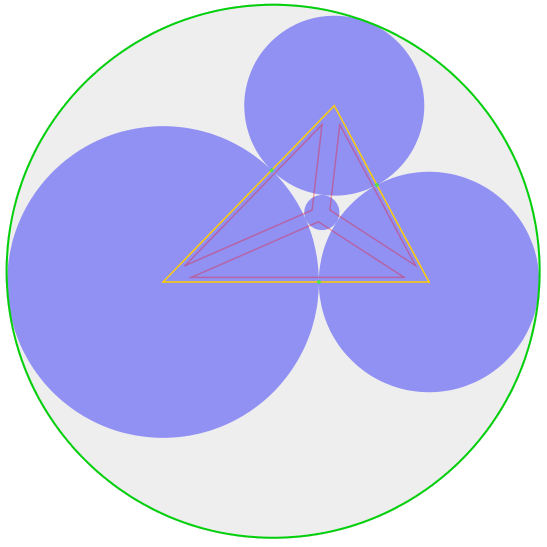
\includegraphics[width=0.65\textwidth]{handleiding-visualisatie-1.png}
  \caption{Voorbeeld visualisatie met drie duidelijke holes} \label{fig:handleiding-visualisatie-1}
\end{figure}

\begin{figure}
  \centering
  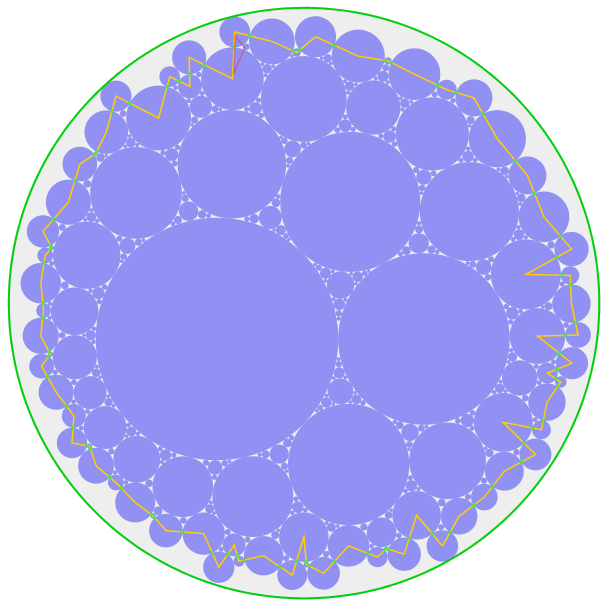
\includegraphics[width=0.65\textwidth]{handleiding-visualisatie-2.png}
  \caption{Voorbeeld visualisatie met grote shell} \label{fig:handleiding-visualisatie-2}
\end{figure}

Deze figuren kan u op de volgende manier interpreteren:

\begin{itemize}  
\item De \textbf{reeds geplaatste cirkels} worden getoond als \textbf{licht blauwe cirkels}.
\item De \textbf{shell} is een \textbf{gele lijn} aan de buitenste rand van de packing. Deze verbind de middelpunten van de cirkels op de shell.
\item De kleine \textbf{groene bolletjes} op de shell geven de posities aan waarop mogelijk een cirkel geplaatst zal worden.
\item \textbf{Holes} worden getoond als \textbf{rode driehoeken}. De hoekpunten liggen dicht bij de middelpunten van de drie cirkels die het gat definiëren.
\item De \textbf{omcirkel} van de huidige packing wordt getoond als een \textbf{groene cirkel}.
\end{itemize}

Op \autoref{fig:handleiding-visualisatie-1} is zijn er duidelijk drie holes te zien.
Elk van de drie holes word gedefinieerd door de centrale cirkel en twee van de buitenste cirkels.
Ook is er een kleine shell te zien, die bestaat uit de buitenste drie cirkels.
In \autoref{fig:handleiding-visualisatie-2} wordt een verder gevorderde packing getoond waarop één hole te zien is, en een veel grotere shell.
Op beide figuren kan je ook de omcirkel zien.

\chapter{Algoritme} \label{chap:algoritme}

In dit hoofdstuk bespreek ik de werking van de heuristiek.
Eerst geef ik een korte beschrijving van het basis idee van het algoritme, gevolgd door de structuur van de code.
Vervolgens leg ik stelselmatig de volledige werking uit, alle veronderstellingen die gemaakt worden en implementatie details waar nodig.
De volledige implementatie is beschikbaar op GitHub \cite{circle-packing-github} en is gebeurd in Java.

Om het algoritme zeer snel te maken worden enkele veronderstellingen gemaakt omtrent de nodige overlap checks bij elke stap.
Deze veronderstellingen zijn niet theoretisch bewezen, maar wel empirisch getest.
Voor de meeste verdelingen van cirkels lijken ze goed stand te houden, maar er zijn nog enkele \textit{edge-cases} waarin er toch nog fouten gebeuren.
Deze problemen worden besproken in \autoref{chap:bedenkingen} en de snelheid en kwaliteit van de oplossingen wordt verder besproken in \autoref{chap:resultaten}.

\section{Basis idee}

Het basis idee van de heuristiek is om stelselmatig een packing op te bouwen, door telkens cirkels te zoeken die het best passen.
Bij elke stap wordt telkens eerst een plek gekozen om een cirkel te plaatsen (in een hole, of op de shell, later hier meer over).
Hier wordt dan de best-passende cirkel geplaatst.
Eenmaal een cirkel geplaatst is wordt deze nooit meer verplaatst.
Dit laat toe om intelligente structuren op te bouwen en deze op een zeer efficiënte manier te gebruiken.

Het algoritme bouwt dus cirkel per cirkel een packing op.
Dit door in elke stap een positie te kiezen, en hierin een cirkel te proberen plaatsen.
Indien er geen cirkel geplaatst kan worden wordt de interne structuur van het probleem vernieuwd om deze nieuwe informatie te reflecteren.
Dit gebeurt op verschillende manieren voor de holes en de shell.
Meer hierover vindt u terug in \autoref{sec:holes} en \autoref{sec:shell}.
Als er wel een cirkel geplaatst kan worden dan wordt deze uit de lijst van nog-te-plaatsen cirkels verwijderd, en krijgt deze een permanente positie daar.
Dit geeft ook aanleiding tot aanpassen van de holes en/of shell.
Hierdoor wordt er een nieuwe tussentijdse packing gemaakt.
Deze wordt dan door gegeven naar de volgende stap, waarin het algoritme opnieuw zal proberen een cirkel te plaatsen.
Op deze manier word een volledige packing opgebouwd voor alle cirkels.

\section{Structuur}

De implementatie van het algoritme bevat enkele belangrijke (programmeer-)klassen die regelmatig zullen terug komen in de verdere uit, vooral in code fragmenten:

\begin{itemize} 
\item Cirkel (Circle)
\item Vector2
\item Locatie (Location)
\item Probleem (Problem)
\item Oplossing (Solution)
\item Oplosser (Solver)
\item Gat (Hole)
\item Schil (Shell)
\end{itemize}

Een $circle$ is voor de hand liggend. Deze heeft een radius, maar geen positie.

$Vector2$ is een 2D positie. Deze bevat een x en y coördinaat.

Een $location$ of locatie is de combinatie van een cirkel met mijn positie. Deze bevat dus een referentie naar een $circle$ en een $vector2$.

Een $problem$ of probleem is een lijst van cirkels.
Deze hebben nog geen positie, en worden gesorteerd van groot naar klein.
Dit is wat de $solver$ als input krijgt.

Een $solution$ of oplossing is een lijst van cirkels met hun positie.
Dit kan een tussen oplossing zijn, waar nog niet voor alle cirkels uit een probleem een positie gevonden is.
Ook geeft dit geen garanties van correctheid, er kan dus bijvoorbeeld overlap zijn, maar voorziet functionaliteit om dit na te gaan.
Dit is wat de solver als output geeft.
Een correcte solver geeft natuurlijk wel altijd goede oplossingen.

Een $solver$ of oplosser is het object dat een packing zoekt voor een gegeven probleem.
Dit is dus het belangrijkste deel van de code, en hier is de nieuwe heuristiek geïmplementeerd.
De best-fit solver, zoals beschreven in deze thesis, doet dit stap voor stap.
In elke stap wordt er één cirkel geplaats op zijn finale positie, dit aan de hand van enkele keuzes die verder in dit hoofdstuk toegelicht zullen worden.

$Hole$ en $shell$ worden verder uitgelegd in respectievelijk \autoref{sec:holes} en \autoref{sec:shell}.

\section{Structuur van de solver}

Zoals hierboven gezegd is de solver het hart van de implementatie.
Deze maakt effectief een packing voor een gegeven probleem.
De solver bevat een lijst van \textit{holes} en de \textit{shell}.
Het bevat ook een lijst van de nog te plaatsen cirkels, en een tussen-oplossing met de cirkels die reeds een plaats gekregen hebben.
Ook heeft hij interne omcirkel voor deze oplossing.
Een oplossing kan zelf ook een omcirkel berekenen, maar de solver gebruikt een interne omcirkel die enkel vernieuwd wordt als het nodig is.
Bovendien heeft de solver extra informatie die de oplossing niet heeft, waardoor deze omcirkel efficiënter berekend kan worden.
Zie \autoref{sec:shell} voor meer uitleg hierover.

In de implementatie ziet de code van de solver er als volgt uit (vereenvoudigde versie):

\begin{lstlisting}
List<Circle> circlesToPack; |\label{code:start-vars}|
Queue<Hole> holes;
List<Location> shell;
Location enclosingCircle;

Solution solution; |\label{code:end-vars}|

void solve() { |\label{code:start-solve}|
	init();
	packFirstThree();
	
	while(!circlesToPack.isEmpty()) { |\label{code:best-fit-loop}|
		boolean ok = bestFitStep();
		if (!ok) break;
	}
}

boolean bestFitStep() {
	if (circlesToPack.isEmpty()) {
		return false;
	}
	
	if(!holes.isEmpty()) {
		...
		// Probeer een cirkel in een gat te plaatsen
		...
		return true;
	}
	else if (!shell.isEmpty()) {
		...
		// Probeer een cirkel op de shell te plaatsen
		...
		return true;
	}
}
\end{lstlisting}

De solver bevat alle nodige informatie over de shell en holes, als ook de cirkels die nog geplaatst moeten worden en de huidige tussen-oplossing (\autoref{code:start-vars} tot \autoref{code:end-vars}).
Om een probleem op te lossen wordt de solve methode (\autoref{code:start-solve}) aangeroepen.
Deze initialiseert eerst alle nodige variabelen, doet dan de initiële packing (meer hierover in \autoref{sec:initialisatie}) en voert dan best-fit-stappen uit tot een oplossing bereikt is (vanaf \autoref{code:best-fit-loop}).

De best-fit solver implementatie uit deze thesis kan stap voor stap de oplossing genereren en tussentijdse oplossingen visualiseren.
Het is dus niet nodig een packing volledig te maken, het kan zeer nuttig zijn tussentijdse oplossingen te zien, zeker bij het debuggen of implementeren van nieuwe functionaliteit.

\section{Initialisatie} \label{sec:initialisatie}

Zoals eerder gezegd bouwt het algoritme steeds verder op een packing uit de vorige stap.
Hierdoor is het dus nodig om een initiële packing te maken van een aantal cirkels waarop de volgende stappen kunnen verder bouwen.
Deze initiële packing is de optimale packing van de drie grootste cirkels in het probleem.
Deze drie cirkels worden zo geplaatst dat ze alle drie aan elkaar raken, zoals getoond in \autoref{fig:initialisatie}.
De licht blauwe cirkels tonen de drie eerste-geplaatste cirkels.
Meer uitleg over hoe u deze figuur kan interpreteren kan u vinden in \autoref{chap:handleiding-visualisaties}

\begin{figure}
  \centering
  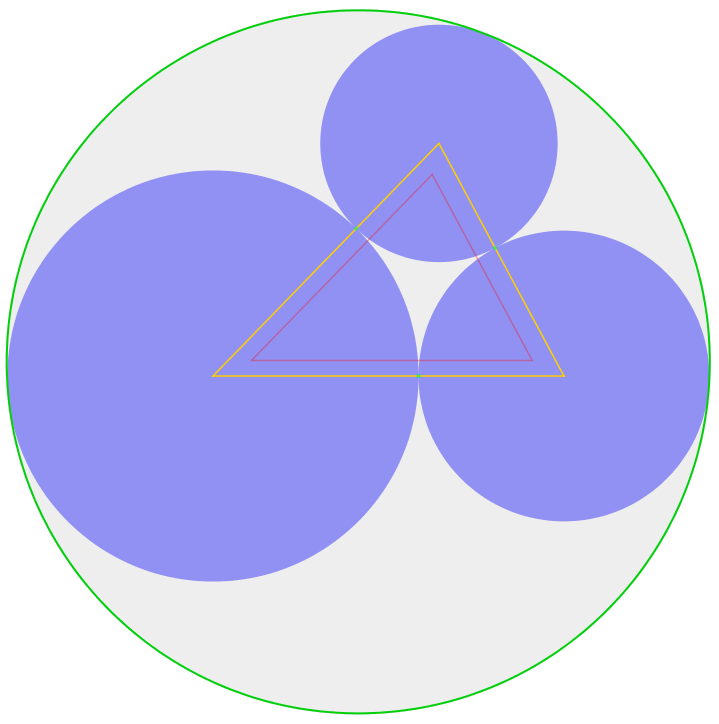
\includegraphics[width=0.65\textwidth]{initialisatie.png}
  \caption{Voorbeeld van initiële packing} \label{fig:initialisatie} 
\end{figure}

Het exacte proces om deze initiële packing te bekomen wordt verduidelijkt aan de hand van code uit de implementatie:

\begin{lstlisting}
private void packFirstThree() {
	//Initially place the two biggest circles next to eachother
	Circle first = circlesToPack.get(0); |\label{code:start-grootste-twee-plaatsen}|
	Circle second = circlesToPack.get(1);

	Vector2 firstPos = new Vector2(0, 0);
	Vector2 secondPos = new Vector2(first.getRadius() + second.getRadius(), 0); |\label{code:end-grootste-twee-plaatsen}|

	Location firstLoc = new Location(firstPos, first);
	Location secondLoc = new Location(secondPos, second);
	getSolution().add(firstLoc); |\label{code:twee-grootste-aan-sol-toevoegen}|
	getSolution().add(secondLoc);

	// Place the third biggest circle on top of the first two (assuming they are positioned clockwise)
	Circle third = circlesToPack.get(2);
	Vector2 thirdPos = Helpers.getMountPositionFor(third, firstLoc, secondLoc); |\label{code:derde-grootste-positie-berekenen}|
	Location thirdLoc = new Location(thirdPos, third);
	getSolution().add(thirdLoc);

	circlesToPack.remove(first);
	circlesToPack.remove(second);
	circlesToPack.remove(third);

	// Create first hole
	holes.add(new NHole(firstLoc, secondLoc, thirdLoc)); |\label{code:eerste-gat-maken}|
	// Create the initial shell
	// IMPORTANT: must be clock-wise
	shell.add(firstLoc); |\label{code:initiele-shell-maken}|
	shell.add(thirdLoc);
	shell.add(secondLoc);

	enclosingCircle = Location.calculateEnclosingCircle(Arrays.asList(firstLoc, secondLoc, thirdLoc));
}
\end{lstlisting}

Eerst worden de twee grootste cirkels naast elkaar geplaatst.
Vanaf \autoref{code:start-grootste-twee-plaatsen} tot \autoref{code:end-grootste-twee-plaatsen} worden eerst de twee grootste cirkels uit het probleem opgevraagd.
De lijst \textit{circlesToPack} is gesorteerd van groot naar klein, dus dit zijn de eerste twee cirkels in deze lijst.
De eerste wordt in de oorsprong geplaatst, en de tweede er tegen op de horizontale as.
Deze worden ook reeds aan de tussentijdse oplossing toegevoegd (vanaf \autoref{code:twee-grootste-aan-sol-toevoegen}).
Vervolgend wordt de positie berekend voor de derde aan de hand van een helper functie op \autoref{code:derde-grootste-positie-berekenen}.
Deze helper functie komt regelmatig terug, en wordt verduidelijkt in \autoref{sec:een-cirkel-tegen-twee-andere-plaatsen}.

In de initialisatie wordt ook het eerste gat gemaakt, gedefinieerd door de eerste drie cirkels.
Dit gat wordt toegevoegd aan de lijst van gaten in de solver op \autoref{code:eerste-gat-maken}.
Ook wordt de shell aangemaakt, vanaf \autoref{code:initiele-shell-maken}.
Deze wordt met de klok mee (gezien vanuit het centrum van de huidige packing) bij gehouden.
Verdere uitleg hierover is te vinden in \autoref{sec:shell}.

\section{Een cirkel tegen twee andere plaatsen} \label{sec:een-cirkel-tegen-twee-andere-plaatsen}

In verschillende delen van de heuristiek is het nodig om een cirkel $c_i$, met radius $r_i$, tegen twee andere cirkels te plaatsen.
Deze twee cirkels noemen we $c_g1, c_g2$, en hun radii $r_g1, r_g2$.
Het punt vinden waarop deze cirkel moet staan om beide andere cirkels te raken wordt bepaald door een eenvoudige cirkel-cirkel intersectie, tussen twee cirkels met hun middelpunt gelijk aan het middelpunt van de cirkels $c_g1$ en $c_g2$ en als radii $r_g1+r_i$ en $r_g2+r_i$:

\begin{lstlisting}
Vector2 getMountPositionFor(Circle cir, Location first, Location second) {
	double x0 = first.getPosition().getX();
	double y0 = first.getPosition().getY();
	double r0 = first.getCircle().getRadius() + cir.getRadius();

	double x1 = second.getPosition().getX();
	double y1 = second.getPosition().getY();
	double r1 = second.getCircle().getRadius() + cir.getRadius();

	// dx en dy zijn de verticale en horizontale afstand tussen de cirkel-centra.
	double dx = x1 - x0;
	double dy = y1 - y0;

	// Bepaalde de afstand tussen de centra
	//d = sqrt((dy*dy) + (dx*dx));
	double d = Math.hypot(dx, dy);

	// 'Punt 2' is het punt waar de lijn door de cirkel-intersectie punten de lijn tussen de cirkel-centra kruist
	// We berekenen hier de coordinaten x2 en y2 van dit punt

	// Bepaal eerst de afstand van tussen Punt 2 en het centrum van de eerste cirkel
	double a = ((r0*r0) - (r1*r1) + (d*d)) / (2.0 * d);

	// Bepaal dan de coordinaten van Punt 2.
	double x2 = x0 + (dx * a/d);
	double y2 = y0 + (dy * a/d);

	// Bepaal nu de afstand van Punt 2 naar een van de intersectie-punten
	// Het tweede intersectie-punt ligt even ver
	double h = Math.sqrt((r0*r0) - (a*a));

	// Zet deze afstand om naar een vector met de juiste richting
	double rx = -dy * (h/d);
	double ry = dx * (h/d);

	// Bepaal een van de tweede intersectie punten
	return new Vector2(x2 - rx, y2 - ry); |\label{code:cirkel-cirkel-intersectie-neg}|
}
\end{lstlisting}

In deze code wordt één van de intersectie punten bepaald.
Dit intersectie punt is steeds het negatieve punt.
Als op \autoref{code:cirkel-cirkel-intersectie-neg} $+$ gebruikt wordt in plaats van $-$ kan het tweede punt bekomen worden.
Het is ook mogelijk het andere intersectie punt te verkrijgen door de twee $location$ parameters om te wisselen.

Het bekomen punt is steeds het punt dat aan uw linker kant zou liggen indien je wandelt van het centrum van de eerste cirkel naar het centrum van de tweede cirkel.
Dit is verduidelijkt in \autoref{fig:cirkel-cirkel-intersectie}, de onderste cirkel is de eerste, de bovenste cirkel de tweede.
De pijl tussen deze cirkels geeft de \textit{wandel richting} aan.

\begin{figure}
  \centering
  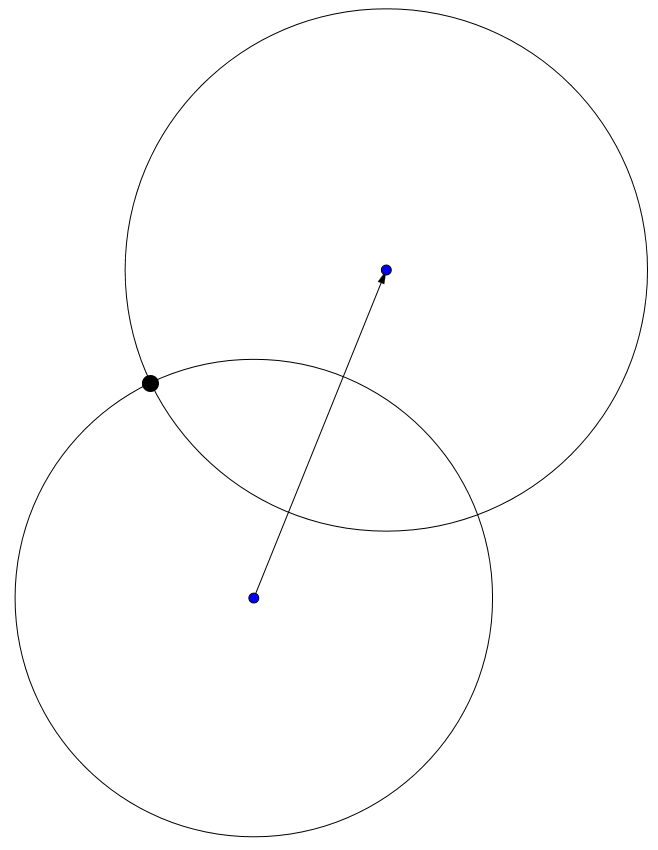
\includegraphics[width=0.65\textwidth]{cirkel-cirkel-intersectie.png}
  \caption{Verkregen intersectie punt van $getMountPositionFor$} \label{fig:cirkel-cirkel-intersectie} 
  \caption*{(Gemaakt met web.geogebra.org)}
\end{figure}

\section{Holes} \label{sec:holes}

Het eerste van de twee belangrijkste concepten van de heuristiek is \textit{holes} of \textit{gaten}.
Dit zijn plaatsen tussen andere, reeds geplaatste, cirkels waar potentieel nog een cirkel tussen kan passen.
De heuristiek zal telkens eerst deze gaten proberen op te vullen, alvorens cirkels op de shell te plaatsen.

Gaten worden gedefinieerd door exact drie cirkels in de huidige packing.
De solver houdt informatie bij voor elk gat waar mogelijk nog een cirkel in kan passen.
Bij elke stap van de solver zal er eerst gekeken worden of er nog gaten in de oplossing zijn.
Indien er nog gaten zijn zal hij deze dus eerst hier een cirkel in proberen plaatsen.
Indien het gat te klein is voor alle nog-te-plaatsen cirkels wordt dit gat simpelweg verwijderd uit de lijst van gaten in de solver.
Op deze manier weet de solver in de volgende stap dat hij daar niet meer moet proberen om een cirkel te plaatsen, en zal hij een ander gat uitproberen.
Indien er wel een cirkel in het gat past wordt deze daar in geplaatst.
Dit zal leiden tot het creëren van drie nieuwe gaten, zoals getoond in \autoref{fig:voorbeeld-gat-stap-1} en \autoref{fig:voorbeeld-gat-stap-2}.
De eerste figuur toont het gat waarin een cirkel geplaatst zal worden (de rode driehoek).
De tweede figuur toont de nieuwe packing, nadat een cirkel geplaatst is in dit gat.
Er zijn drie nieuwe kleinere gaten gemaakt, die in de volgende stappen ook zullen opgevuld worden indien mogelijk.
Het algoritme zal deze gaten ook terug proberen opvullen.
In \autoref{fig:voorbeeld-gat-stap-3} en \autoref{fig:voorbeeld-gat-stap-3alt} wordt respectievelijk de tussen-oplossing getoond voor wanneer er nog een cirkel is die klein genoeg is, en wanneer dit niet het geval is, om het onderste gat op te vullen.

\begin{figure}
  \centering
  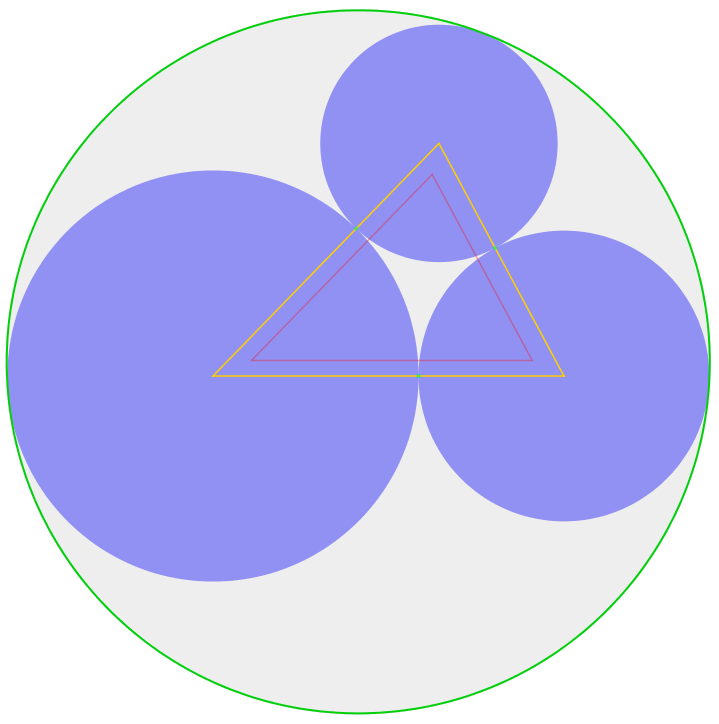
\includegraphics[width=0.65\textwidth]{voorbeeld-gat-stap-1.png}
  \caption{Packing voor het opvullen van een gat} \label{fig:voorbeeld-gat-stap-1} 
\end{figure}

\begin{figure}
  \centering
  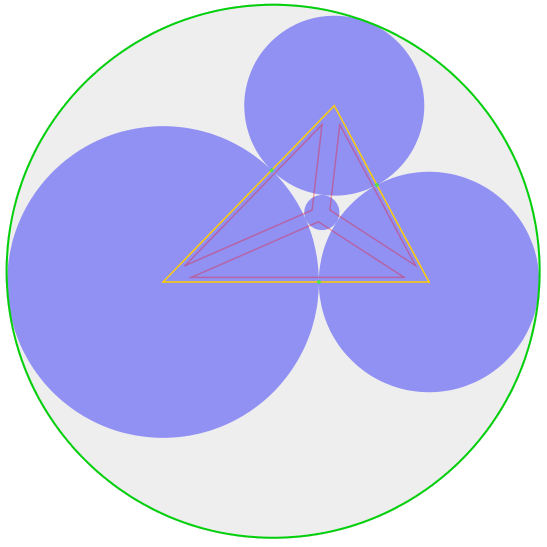
\includegraphics[width=0.65\textwidth]{voorbeeld-gat-stap-2.png}
  \caption{Packing na het opvullen van een gat} \label{fig:voorbeeld-gat-stap-2} 
\end{figure}

\begin{figure}
  \centering
  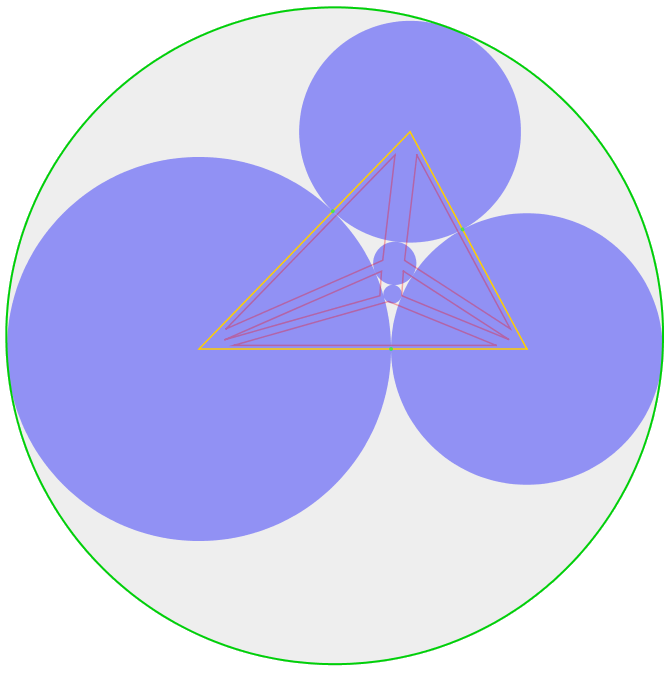
\includegraphics[width=0.65\textwidth]{voorbeeld-gat-stap-3.png}
  \caption{Packing na het opvullen van een tweede gat} \label{fig:voorbeeld-gat-stap-3} 
\end{figure}

\begin{figure}
  \centering
  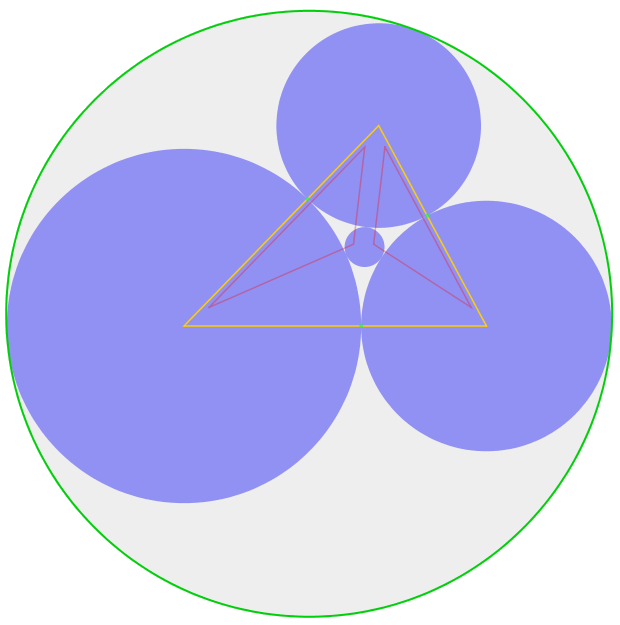
\includegraphics[width=0.65\textwidth]{voorbeeld-gat-stap-3alt.png}
  \caption{Packing als het opvullen van een tweede gat mislukt} \label{fig:voorbeeld-gat-stap-3alt} 
\end{figure}

\subsection{Grootste cirkel zoeken die past in een \textit{hole}} \label{sec:grootste-cirkel-zoeken-die-past-in-een-hole}

Bij het plaatsen van een cirkel in een gat wordt een zo groot mogelijke cirkel gezocht die in dit gat past.
Dit is bij wijze van spreken de best-passende cirkel, vandaar \textit{best-fit}.
Meer uitleg over hoe bepaald wordt of een cirkel past vind je in \autoref{subsec:bepalen-of-een-cirkel-past-in-hole}.
Hier wordt het proces om te vinden \textit{welke} cirkel past verder verduidelijkt.
Er wordt binair gezocht door de lijst van cirkels om te bepalen welke cirkel de grootste is die past.
Onderstaande code verduidelijkt dit proces.

\begin{lstlisting}
Location findBestFitFor(Hole hole, List<Circle> sortedBigToSmall) {
	// Probeer eerst de kleinste cirkel
	int lower = sortedBigToSmall.size() - 1; |\label{code:probeer-eerst-kleinste-in-hole}|
	Circle smallestCir = sortedBigToSmall.get(lower);
	Vector2 smallestPos = hole.tryFit(smallestCir);
	if (smallestPos == null) {
		return null;
	}

	// Probeer dan de grootste cirkel
	int upper = 0; |\label{code:probeer-dan-grootste-in-hole}|
	Circle biggestCir = sortedBigToSmall.get(upper);
	Vector2 biggestPos = hole.tryFit(biggestCir);
	if (biggestPos != null) {
		return new Location(biggestPos, biggestCir);
	}

	// Binair zoeken
	Circle cir = null;
	Vector2 pos = null;
	while (lower - upper > 1) {
		int middle = (upper + lower) / 2;
		cir = sortedBigToSmall.get(middle);
		pos = hole.tryFit(cir);

		if (pos == null) {
			upper = middle;
		}
		else {
			lower = middle;
		}
	}

	cir = sortedBigToSmall.get(lower);
	pos = hole.tryFit(cir);
	if (pos != null) {
		return new Location(pos, cir);
	}
	else {
		return null;
	}
}
\end{lstlisting}

De solver houdt de lijst van cirkels bij gesorteerd op grootte, dat is cruciaal om snel de beste-passende cirkel te vinden.
Eerst worden de grootste en kleinste cirkel uitgeprobeerd (\autoref{code:probeer-eerst-kleinste-in-hole}).
Indien de kleinste niet past zal het algoritme direct rapporteren dat dit gat te klein is.
Het gat zal dan, zoals vermeld in \autoref{sec:holes}, verwijderd worden uit de lijst van mogelijk holes.
Indien de grootste past (\autoref{code:probeer-dan-grootste-in-hole}) zal het algoritme onmiddellijk deze cirkel plaatsen in het gat.
Er zijn immers geen grotere cirkels, dus deze is de cirkel die verondersteld wordt best te passen.
Vervolgens word er een gebied bepaald in de overblijvende cirkels, waarin de best-passende cirkel zich bevind.
Initieel ligt de boven-en ondergrens van dit gebied op de uiteinden van de overblijvende cirkels.
De cirkel in de midden van dit gebied wordt dan uitgeprobeerd.
Afhangende of deze wel of niet past zal de boven-of ondergrens aangepast worden.
Dit wordt telkens herhaald tot er nog maar één cirkel over blijft.
Dit is dan de grootste cirkel die past in het gat.

\subsection{Bepalen of een cirkel past in een \textit{hole}} \label{subsec:bepalen-of-een-cirkel-past-in-hole}

Er is geen exact definitie van de grootte van een gat.
Dit is niet mogelijk omdat de cirkels die het gat bepalen niet altijd aan elkaar raken.
Het is echter wel mogelijk om te bepalen of een cirkel past.

Dit gebeurt door de cirkel die we willen testen te plaatsen in het gat.
Eerst wordt de cirkel tegen twee van de cirkels in het gat geplaatst, met een cirkel-cirkel intersectie zoals beschreven in \autoref{sec:een-cirkel-tegen-twee-andere-plaatsen}.
Deze cirkel-cirkel intersectie heeft natuurlijk altijd twee punten.
Hiervan moet er één gekozen worden.
De implementatie zorgt er voor dat de cirkels die het gat definieren telkens tegen de klok gesorteerd zijn (ten op zichte van het middelpunt van deze deze drie cirkels).
Dit maakt het mogelijk telkens het juiste punt te kiezen.
Eenmaal dit punt bepaald is word de cirkel op deze plek gezet.
Dan wordt gekeken of deze cirkel wel effectief in het gat geplaatst is, en of deze niet overlapt met de derde cirkel die het gat definieert.

\begin{lstlisting}
public Vector2 tryFit(Circle cir) {
	// Try to place circle
	Vector2 pos = Helpers.getMountPositionFor(cir, first, second);

	// Check that is inside the hole
	boolean inside = Vector2.isInsideTriableBy(first.getPosition(), second.getPosition(), third.getPosition(), pos); |\label{code:try-fit-in-triangle}|
	if (!inside) {
		return null;
	}

	// Test for overlap
	Location loc = new Location(pos, cir);
	if (third.overlaps(loc)) { |\label{code:try-fit-derde-overlap}|
		return null;
	}
	return pos;
}
\end{lstlisting}

Op \autoref{code:try-fit-in-triangle} wordt verzekerd dat het middelpunt van de cirkel in het gat ligt.
Dit voorkomt dat de geplaatste cirkel buiten het gat geplaatst wordt, en dus zeker niet kan overlappen met cirkels buiten het gat zonder ook te overlappen met één van de cirkels die het gat definiëren.
Op \autoref{code:try-fit-derde-overlap} wordt dan de overlap met de derde gat-definiërende cirkel nagekeken.
Er kan geen overlap zijn met de eerste twee, de methode $getMountPositionFor$ plaatst de cirkel zodanig dat deze de twee andere cirkels raakt, maar niet overlapt.
Indien de cirkel in het gat past, en dus alle checks doorstaat, wordt de positie voor deze cirkel terug gegeven.
De solver zal deze cirkel dan plaatsen in zijn oplossing.

Het is niet nodig om na te gaan of er overlap is met andere cirkels in de oplossing.
Als er met een andere overlap zou zijn, moet dit zijn omdat de cirkel buiten het gat geplaatst is, of er is ook overlap met één van de cirkels in het gat zelf.
Dit zorgt er voor dat er zeer weinig overlap-checks gedaan moeten worden, wat het algoritme zeer snel maakt.

\section{Shell} \label{sec:shell}

De \textit{shell} of \textit{schil} is het tweede van de belangrijkste concepten van de heuristiek.
Dit is de buitenste laag van cirkels in een (tussen-)oplossing van de solver.
Deze wordt in de implementatie simpelweg bijgehouden als een geordende lijst van cirkels.
Cirkels die naast elkaar staan in de lijst, grenzen ook aan elkaar in de shell.
De cirkels in deze laag zijn met de klok mee gesorteerd, ten opzichte van het middelpunt van de omcirkel.
De eerste en laatste cirkel in de lijst grenzen ook aan elkaar in de shell.

De heuristiek voorgesteld in deze thesis probeert steeds eerst alle gaten op te vullen.
Maar wanneer er geen cirkels meer over zijn die klein genoeg zijn om te passen in gaten, word er een cirkel op de shell geplaatst.
Op de shell worden alle posities tegen twee cirkels van de shell overwogen.
Dit is een goede heuristiek voor de optimale positie, beperkt het aantal mogelijke posities voor de geplaatste cirkel enorm en maakt het algoritme dus zeer snel (zie \autoref{chap:resultaten} voor een vergelijking in snelheid).
Er wordt steeds een cirkel zo dicht mogelijk bij het centrum van de huidige tussen-oplossing geplaatst.
Dit om het uitbreiden van de omcirkel zo min mogelijk te houden.

Eerst worden twee cirkels gekozen waartegen de nieuwe geplaatst zal worden.
Hiervoor wordt gekeken naar het middelpunt tussen alle cirkels die naast elkaar staan op de shell.
De twee cirkels waarvoor het middelpunt het dichtst bij het centrum van de huidige omcirkel ligt worden gekozen als kandidaten om de derde cirkel tegen te plaatsen.
Dan wordt er gezocht naar een zo groot mogelijke cirkel die daar past op de shell.
Indien geen enkele cirkel past wordt één van de twee kandidaat cirkels verwijderd uit de shell.
Welke verwijderd wordt verduidelijkt in \autoref{sec:bepalen-of-een-cirkel-past-op-de-shell}.
Dit zorgt er voor dat de shell verandert en \textit{groeit} naar buiten.
In de volgende stap van het algoritme zal dan ook een andere positie voor een cirkel uitgeprobeerd worden.
Indien er wel een cirkel past wordt deze toegevoegd aan de shell, en geeft deze aanleiding tot een nieuw gat.
Dit gat zal vervolgens opgevuld worden indien mogelijk, zoals beschreven in \autoref{sec:holes}.
Op \autoref{fig:plaats-op-shell-simpel} wordt getoond hoe de packing verandert wanneer een cirkel geplaatst wordt op de shell.
Eerst wordt een packing zonder gaten getoond en vervolgens de packing nadat een cirkel op de shell geplaatst is.
Hierop is duidelijk te zien hoe de shell aangepast is geweest, en deze plaatsing geleid heeft tot een nieuw gat.
Zoals eerder gezegd is het mogelijk dat op een positie op de shell de grootste cirkel niet past.
Dit wordt geïllustreerd in \autoref{fig:plaats-op-shell-kleiner}.
Het is ook mogelijk dat geen enkele cirkel nog past op de shell, zoals getoond in \autoref{fig:plaats-op-shell-geen-enkele-past}.

\begin{figure}
  \centering
  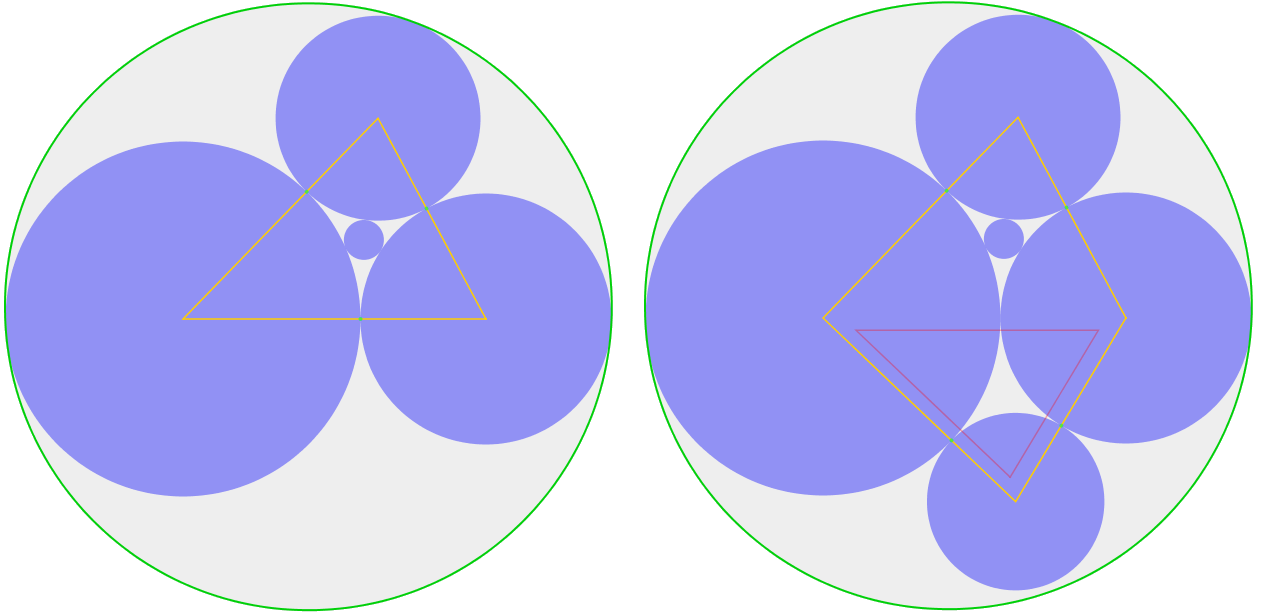
\includegraphics[width=1.0\textwidth]{plaats-op-shell-simpel.png}
  \caption{Het plaatsen van de grootste cirkel op de shell} \label{fig:plaats-op-shell-simpel} 
\end{figure}

\begin{figure}
  \centering
  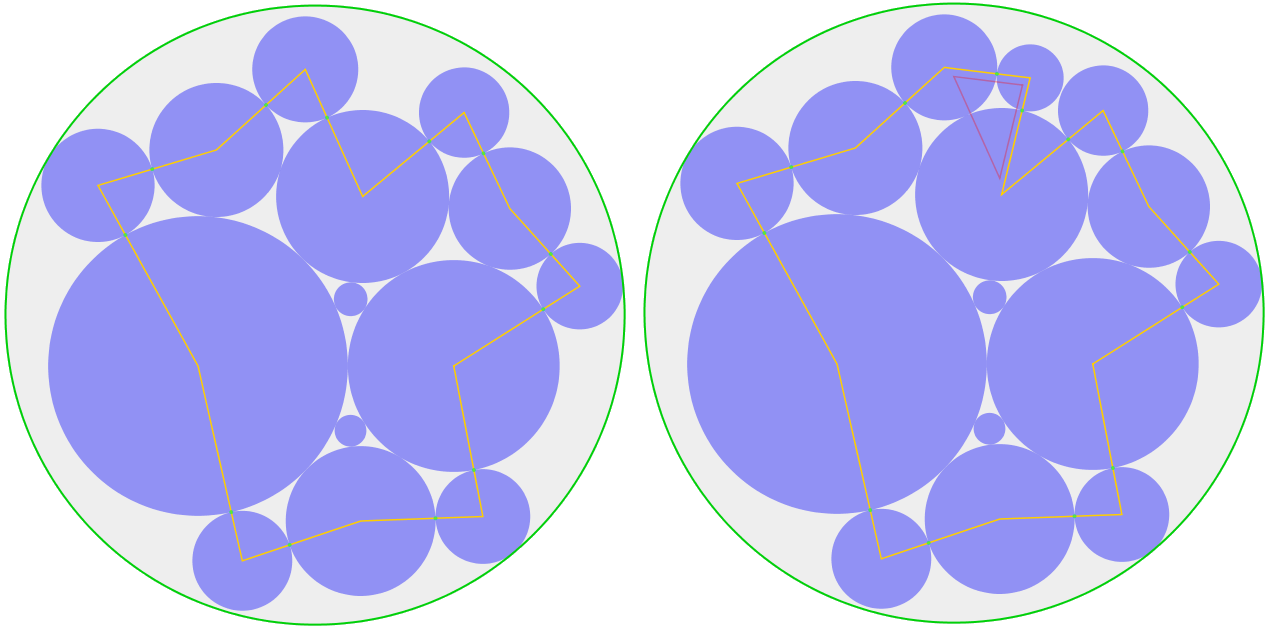
\includegraphics[width=1.0\textwidth]{plaats-op-shell-kleiner.png}
  \caption{Het plaatsen van een kleinere cirkel op de shell} \label{fig:plaats-op-shell-kleiner} 
  \caption*{Focus: midden bovenaan}
\end{figure}

\begin{figure}
  \centering
  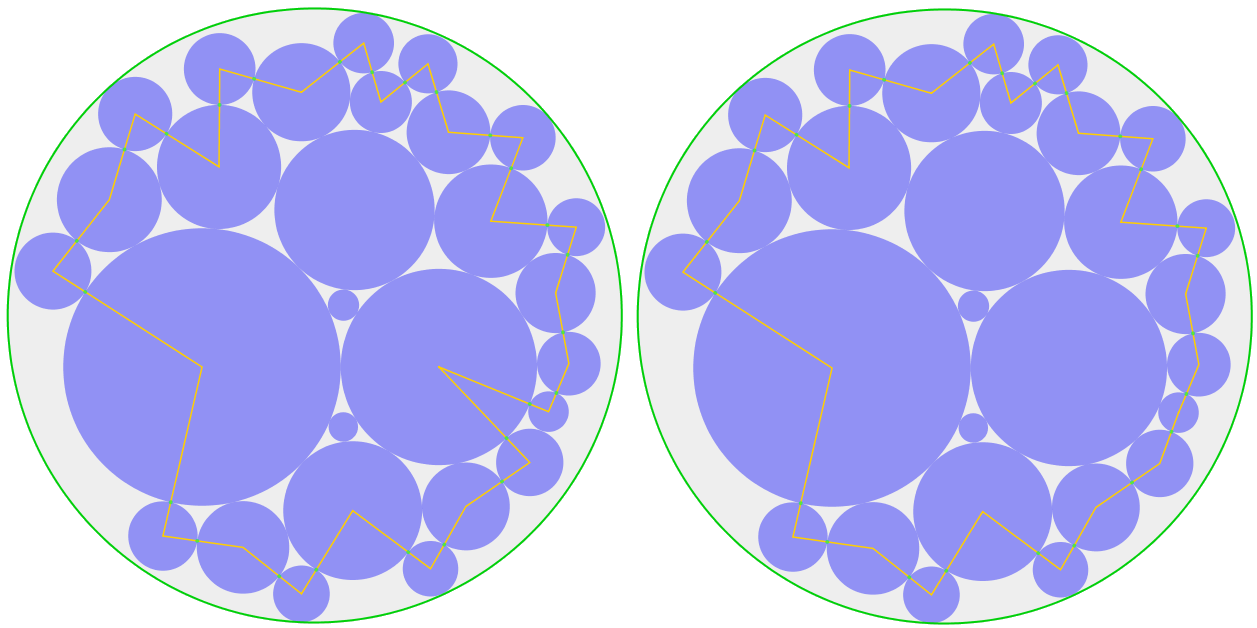
\includegraphics[width=1.0\textwidth]{plaats-op-shell-geen-enkele-past.png}
  \caption{Shell aanpassen als geen enkele cirkel past} \label{fig:plaats-op-shell-geen-enkele-past} 
  \caption*{Focus: rechts onderaan}
\end{figure}

\subsection{Slim de omcirkel berekenen gebaseerd op de shell}

Bij het kiezen van de kandidaat cirkels om een cirkel tegen te plaatsen op de shell wordt gebruik gemaakt van de omcirkel van de huidige tussen-oplossing.
Zoals eerder vermeld kan voor elke (tussen-)oplossing de omcirkel berekend worden.
Dit gebeurt door een aangepaste versie van het Welz algoritme voor de omcirkel van punten beschreven in \cite{welzl1991smallest}.
De implementatie is gebaseerd op de implementatie in \cite{sunshine2008welzl}.
Het is een recursief algoritme dat in lineaire tijd de omcirkel kan berekenen.
Het idee is dat de omcirkel van een aantal cirkels (of punten) volledig gedefinieerd is door maximum drie cirkels.
Het algoritme vind deze twee of drie cirkels.

Het is eenvoudig in te zien dat deze drie cirkels aan de buitenkant van een (tussen-)oplossing zullen liggen.
Dit is ook net wat de shell is, de cirkels aan de buitenkant van een oplossing.
Het is dus mogelijk om in elke stap van de solver de omcirkel zeer efficient te berekenen.
De complexiteit is dan slechts lineair in het aantal cirkels op de shell in huidige (tussen-)oplossing, wat slechts een subset is van totaal aantal cirkels in de oplossing.
Aangezien de omcirkel regelmatig moet herberekend worden doorheen het algoritme is dit een zeer interessante optimalisatie.

\subsection{Bepalen of een cirkel past op de shell} \label{sec:bepalen-of-een-cirkel-past-op-de-shell}

Om te bepalen of een cirkel op de shell past plaatsen we de cirkel eerst tegen twee cirkels op de shell.
Dit gebeurt op de zelfde manier als het plaatsen van een cirkel tegen twee cirkels van een gat.
De exacte methode is reeds uitgelegd in \autoref{sec:een-cirkel-tegen-twee-andere-plaatsen}.
Eenmaal deze positie gekend is, wordt er nagekeken of dit niet tot overlap leidt.
Indien er overlap is is het niet mogelijk om de cirkel daar op de shell te plaatsen, en wordt er informatie terug gegeven over welke cirkel op de shell voor problemen zorgt.

Om na te gaan of er overlap is, wordt er systematisch een aantal cirkels op de shell nagekeken.
Het is niet nodig andere cirkels, die niet op de shell zitten, na te kijken voor overlap.
Een nieuwe cirkel wordt steeds op de shell geplaatst zodanig dat als er overlap zou zijn met cirkels in de oplossing, minstens één van die cirkels op de shell ligt.
Doordat ik geen exacte definitie van de shell heb, ze is enkel gedefinieerd door het algoritme dat ze opbouwt, is het niet mogelijk om hier een echt bewijs van te geven.
Uit empirische tests lijkt dit echter wel te kloppen.
Verdere bedenkingen hierbij kan u terug vinden in \autoref{chap:bedenkingen}.
Om deze overlappings-test zeer snel te kunnen uitvoeren worden eerst cirkels dicht bij nagekeken.
Er staat ook een limiet op het aantal cirkels die getest worden.
Uit tests, tot 5000 cirkels, blijkt dat drie cirkels aan elke kant van de shell nakijken genoeg is.
Voor de meeste gevallen is één cirkel nakijken genoeg, maar sommige randgevallen (wanneer meerdere kleine cirkels dicht bij elkaar staan op de shell) vragen deze extra checks.

Het aantal cirkels dat nagekeken wordt is een hyperparameter $checkRadius$ van het algoritme.
De volgende code toont hoe de overlap nagekeken wordt:

\begin{lstlisting}
for (int i = 1; i <= checkRadius; ++i) {
	int prevIndex = (firstIndex + shell.size() - i) % shell.size();
	Location prev = shell.get(prevIndex);
	if (loc.overlaps(prev)) {
		toRemove = first;
		break;
	}
	int nextIndex = (secondIndex + i) % shell.size();
	Location next = shell.get(nextIndex);
	if (loc.overlaps(next)) {
		toRemove = second;
		break;
	}
}
\end{lstlisting}

Er wordt dus om te beurt links en rechts van de huidige positie op de shell nakeken voor overlap.
Indien er overlap gevonden is, wordt bijgehouden aan welke kant van de shell dit gebeurd is.
$toRemove$ is dus uiteindelijk $first$ of $secons$, wat aan geeft of er aan de kant van de eerste cirkel, of van de tweede cirkel, overlap voorkomt.
$toRemove$ kan ook $null$ zijn indien er geen overlap is.
Deze informatie wordt dan gebruikt door de solver om te bepalen of de cirkel geplaatst kan worden ($toRemove = null$), of dat de shell aangepast moet worden.
Meer informatie hierover in \autoref{sec:een-cirkel-plaatsen-op-de-shell}

\subsection{Een cirkel plaatsen op de shell} \label{sec:een-cirkel-plaatsen-op-de-shell}

Om een cirkel te plaatsen op de shell wordt eerst de grootste cirkel is die past op de shell binair gezocht in de lijst van nog-te-plaatsen cirkels.
Dit gebeurt op analoge manier als het zoeken naar de grootste cirkel die past in een gat, zoals beschreven in \autoref{sec:grootste-cirkel-zoeken-die-past-in-een-hole}.
Indien er een cirkel gevonden wordt die past op de shell wordt de shell uitgebreid met deze cirkel.
De cirkel wordt dan tussen de cirkels, waartegen hij geplaatst is, gezet in de shell.
Dit wordt geïllustreerd in \autoref{fig:plaats-op-shell-simpel}, \autoref{fig:plaats-op-shell-kleiner}.
De gele lijn (die de shell voorstelt, zoals beschreven in \autoref{chap:handleiding-visualisaties}) wordt uitgebreid met een extra punt.
Ook zorgt dit er voor dat een nieuw gat gemaakt wordt waar mogelijk kleinere cirkels in passen.

Een laatste check die gebeurt is om na te gaan of door het plaatsen van de cirkel de shell nog juist gevormd is.
Indien een cirkel geplaatst wordt zodat de cirkels niet meer met de klok mee gesorteerd zijn, zou dit er voor kunnen zorgen dat foutieve plaatsingen voorkomen.
Om dit te voorkomen wordt de gerichte hoek tussen de geplaatste cirkel en de cirkels waartegen hij geplaatst is nagekeken.
Indien deze hoek negatief is wordt de shell hier voor aangepast.
Dit wordt getoond in \autoref{fig:plaats-op-shell-hoek}.
Het eerste deel toont de configuratie waarop een cirkel geplaatst zal worden.
Het laatste deel de uiteindelijke configuratie van de shell.
Het middelste deel toont met een zwarte lijn het deel van de shell dat verwijderd is om er voor te zorgen dat deze kloksgewijs gesorteerd blijft.
Op \autoref{fig:plaats-op-shell-hoek-fout}  wordt getoond wat er kan gebeuren als deze check niet gebeurt.

\begin{figure}
  \centering
  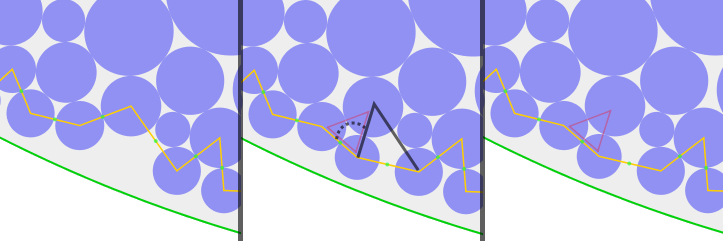
\includegraphics[width=1.0\textwidth]{plaats-op-shell-hoek.png}
  \caption{Een cirkel veroorzaakt een tegen-ge-klok shell} \label{fig:plaats-op-shell-hoek} 
\end{figure}

\begin{figure}
  \centering
  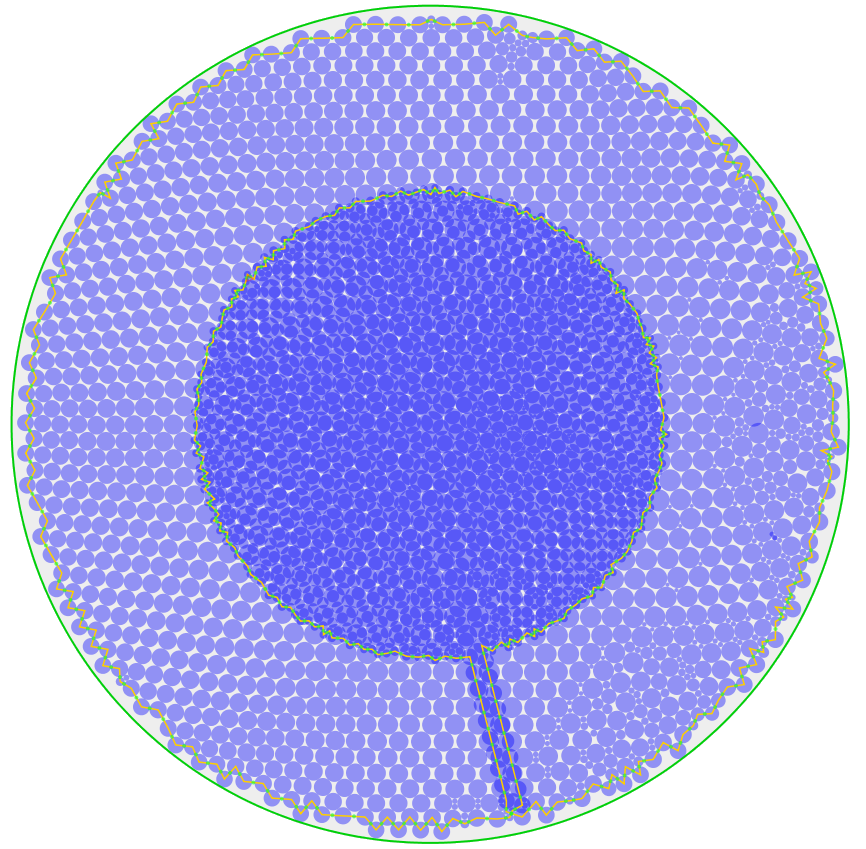
\includegraphics[width=.65\textwidth]{plaats-op-shell-hoek-fout.png}
  \caption{Mogelijke fout indien de shell niet met de klok mee gesorteerd is} \label{fig:plaats-op-shell-hoek-fout} 
\end{figure}

\section{Conclusie}

Dit hoofdstuk gaf een volledig overzicht van de nieuwe constructieve heuristiek.
Waar nodig werd het uitleg verduidelijkt met code uit de implementatie.
Er werden ook de verschillende veronderstellingen geformuleerd die gebruikt worden om het algoritme zeer snel te maken.
Zie ook \autoref{chap:bedenkingen} voor verdere bedenkingen hieromtrent.


\chapter{Bedenkingen bij implementatie} \label{chap:bedenkingen}

\section{Precisie}

De implementatie gebruikt $double$ variabelen.
Ook geeft de methode gebruikt om cirkels tegen elkaar te plaatsen, beschreven in \autoref{sec:een-cirkel-tegen-twee-andere-plaatsen}, geen exacte oplossing.
Hierdoor wordt er doorheen het algoritme een kleine fout opgebouwd.
Deze fout uit zich in een kleine overlap in de uiteindelijke verkregen packing.
Deze overlap blijft echter beperkt tot $10^{-15}$ vierkante eenheden voor de grootste packings.

Dit is een inherent probleem van werken in eindige precisie.
Andere algoritmen hebben dus te kampen met het zelfde probleem, hoewel er niet altijd aandacht aan wordt besteed in de gepubliceerde papers.
In \cite{akeb2006basic}, \cite{ye2013iterated} en \cite{m2013packing} worden resultaten verkregen met een precisie van respectievelijk $10^{-10}$, $10^{-28}$ en $10^{-7}$.

%\cite{akeb2006basic} -> $10^{-10}$.
%\cite{ye2013iterated} -> $10^{-28}$.
%\cite{m2013packing}  -> $10^{-7}$.

Aangezien de vergelijkingen in \autoref{chap:resultaten} tot een precisie van $10^{-10}$ gebeuren heeft dit verder geen impact op de resultaten.

\section{Veronderstellingen}

Zoals eerder vermeld worden er, bij de gaten en shell, enkele veronderstellingen gedaan om het algoritme zeer snel te laten verlopen.
Deze veronderstellingen lijken voor de meeste problemen correct te zijn.
Er zijn echter sommige problemen, vooral als er gewerkt wordt met zeer hoge aantallen cirkels (duizenden), dat er toch nog fouten kunnen gebeuren.
Dit uit zich dan in packings met een grote overlap.

Uit huidige tests lijkt er vooral een probleem met de gaten, de shell heeft voor zover mijn huidige tests uitwijzen geen problemen.
Doordat de cirkels die een gat definiëren niet altijd aan elkaar raken kan het gebeuren, als twee gaten naast elkaar staan, er toch nog een overlap is.

Een voorstel om dit op te lossen is een gat niet op te delen in drie gaten als er een cirkel in geplaatst wordt, maar slechts in twee.
Eén van die gaten bestaat dan uit meer dan drie cirkels.
Zo is het wel mogelijk om altijd aaneensluitende cirkels een gat te laten bepalen.

\chapter{Resultaten} \label{chap:resultaten}

In dit hoofdstuk worden de verkregen packings vergeleken met de best gekende packings, zoals gerapporteerd op de Packomania website \cite{packomania}.
Packomania is een website die de best gekende oplossingen voor verschillende circle-packing problemen verzameld.
Deze vergelijking wordt gemaakt op zowel de verkregen radius van de omschreven cirkel, als ook de tijd nodig om tot deze packing te komen indien deze gekend is.
De nodige rekentijd voor deze algoritmen is echter niet altijd even makkelijk te vinden.
Veel van de packings op Packomania hebben geen bijhorende publicatie.
Het gebruikte algoritme en de nodige tijd om de packing te bekomen is dus niet gekend, enkel de verkregen omschreven cirkel en coördinaten van de packing.
De vergelijking in tijd zal dus een zeer ruwe vergelijking zijn gebaseerd op slechts enkele papers.

Ook geef ik resultaten voor packings met veel meer cirkels dan deze geraporteerd op Packomania.
Hiervoor heb ik geen andere resultaten gevonden in de literatuur om met te vergelijken.

Packomania heeft resultaten voor verschillende verdelingen van cirkels.
Deze verdelingen zijn als volgt:

\begin{itemize}
	\item $r_i=1$ (alle cirkels gelijke grootte)
	\item $r_i=i$
	\item $r_i=i^{1/2}$
	\item $r_i=i^{-1/5}$
	\item $r_i=i^{-1/2}$
	\item $r_i=i^{-2/3}$
\end{itemize}

Hierbij zijn er telkens $N$ cirkels in het probleem, en is $i \in (1,2,...,N)$.
De verhouding tussen enkele van deze verdelingen worden verduidelijk in \autoref{fig:packomania-verdelingen}.

\begin {figure}
	\centering
	\resizebox {0.8\columnwidth} {!} {
		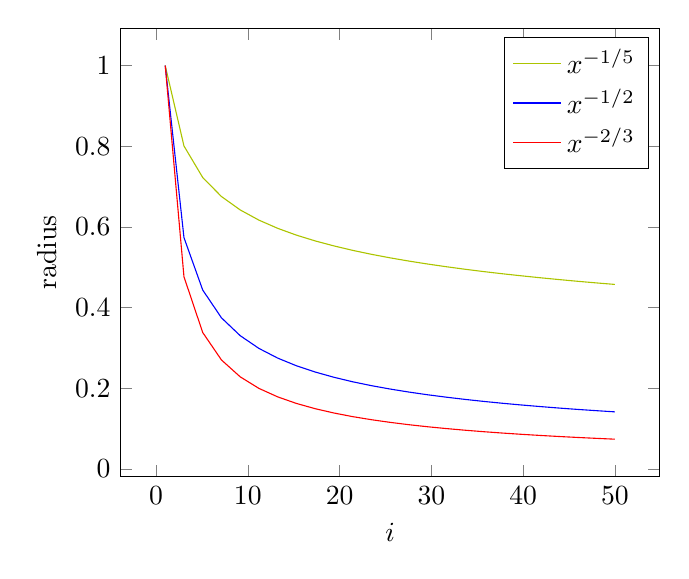
\begin{tikzpicture}
			\begin{axis}[ xlabel=$i$, ylabel=radius, domain=1:50 ]
				\addplot[green]{x^(-1/5)};
				\addlegendentry{$x^{-1/5}$}
				
				\addplot[blue]{x^(-1/2)};
				\addlegendentry{$x^{-1/2}$}
				
				\addplot[red]{x^(-2/3)};
				\addlegendentry{$x^{-2/3}$}
			\end{axis}
		\end{tikzpicture}
	}
	\caption{Packomania verdelingen}
	\label{fig:packomania-verdelingen}
\end {figure}

Al deze berekeningen zijn uitgevoerd op een Mid 2009 Macbook-Pro 15 inc met een 2.8Ghz Core 2 Duo processor en 4GB ram.

\section{Packomania vergelijking}

\subsection{Even grote cirkels}

In \autoref{fig:vergelijking-even-grote-cirkels} wordt de procentuele vergroting weergegeven voor packings met $N$ cirkels van gelijke grootte.
Er wordt een volledig beeld gegeven, als ook een detail-beeld waar vergrotingen boven de 1,5\% niet worden getekend.
Deze vergroting is ten opzichte van de best gekende oplossing op de Packomania website.
Tabellen die mijn resultaten met de best gekende vergelijken kan u terug vinden in \autoref{append:packomania-tabellen-gelijke-grootte}.

\begin {figure}
	\centering
	\resizebox {0.8\columnwidth} {!} {
		\begin{tikzpicture}
			\begin{axis}[xlabel=Aantal Cirkels, ylabel=\% Vergroting]
				\addplot table [x=N, y=Increase, col sep=comma]{csv/Equal size Packomania problems comparison.csv};
				\addlegendentry{Gelijke grootte}
			\end{axis}
		\end{tikzpicture}
	}
	\resizebox {0.8\columnwidth} {!} {
		\begin{tikzpicture}
			\begin{axis}[xlabel=Aantal Cirkels, ylabel=\% Vergroting, ymin=0, ymax=1.5]
				\addplot table [x=N, y=Increase, col sep=comma]{csv/Equal size Packomania problems comparison.csv};
				\addlegendentry{Gelijke grootte}
			\end{axis}
		\end{tikzpicture}
	}
	\caption{Vergelijking van packings van even grote cirkels}
	\label{fig:vergelijking-even-grote-cirkels}
\end {figure}

Gemiddeld geeft mijn algoritme een resultaat dat $0,79\%$ groter is dan de het best gekende resultaat voor problemen met cirkels van gelijke grootte.
Er is echter een duidelijke neerwaartse trend.
Voor problemen met meer dan 1000 cirkels is de gemiddelde vergroting nog slechts 0,48\%.
Voor meer dan 2000 cirkels nog 0,39\% en voor meer dan 3000 nog 0,32\%.
Problemen met een groter aantal cirkels geven duidelijk een beter resultaat.

Dit komt mogelijk omdat hoe meer cirkels er zijn, hoe moeilijker het probleem wordt.
Hierdoor zullen de best-gekende oplossingen voor problemen met zulke grote aantallen cirkels minder dicht bij de absolute optimale oplossing liggen.
Omdat mijn algoritme enkel nieuwe cirkels tegen twee reeds geplaatste cirkels plaats, hebben al mijn oplossingen voor dit probleem een duidelijke structuur.
Deze structuur is een zeshoekige structuur.
Dit wordt geïllustreerd in \autoref{fig:packing-even-groot-50}.
Dit is een zeer eenvoudige structuur, maar lijkt toch redelijk goed de best gekende oplossingen te benaderen.
Meer figuren hiervan vind u terug in \autoref{append:extra-packing-figuren}.

Nodige tijd blijft onder 10 milliseconden tot $N=100$.
Tot 500 cirkels blijft de nodige rekentijd onder 100 milliseconden.
De rekentijd loopt pas op tot één seconde bij 2200 cirkels, en slechts 3,5 seconden voor 5000 cirkels.

Zoals eerder vermeld zijn vergelijkingen in nodige rekentijd moeilijk te vinden.
In \cite{grosso2010} worden echter tijden gerapporteerd van 110 seconden voor 30 cirkels (mijn algoritme vroeg hier minder dan een millisecond tijd), en 15311 seconden (meer dan 4 uur) voor 100 cirkels (mijn algoritme vroeg hier 7 milliseconden).
Zij halen resultaten die zeer dicht bij de best gekende liggen (soms de beste).

Zelfs de constructieve algoritmen beschreven in \cite{akeb2006basic} en \cite{hifi2004approximate} vragen meerdere seconden, en soms minuten, om te berekenen.
Hun resultaten zijn echter moeilijk te vergelijking omdat \cite{akeb2006basic} een alternatieve versie van circle-packing oplost, en \cite{hifi2004approximate} packings maakt in rechthoeken.

\begin{figure}
  \centering
  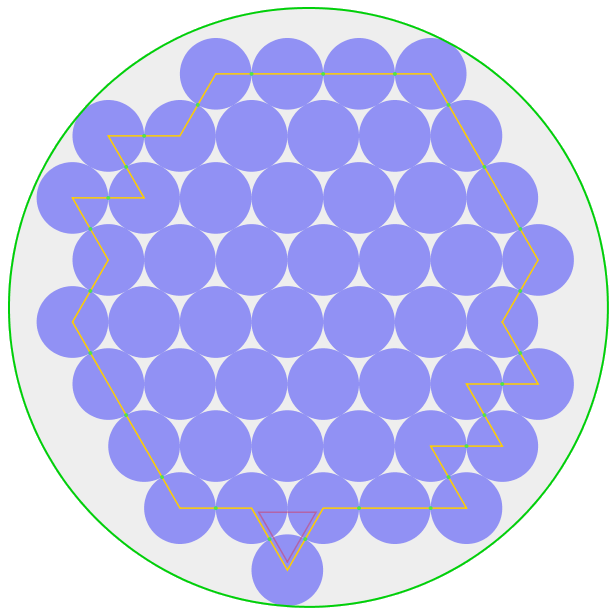
\includegraphics[width=0.65\textwidth]{packing-even-groot-50.png}
  \caption{Packing voor 50 even grote cirkels} \label{fig:packing-even-groot-50} 
\end{figure}

\subsubsection{Bespreking}

Over het algemeen zijn dit goede resultaten.
Ze liggen redelijk dicht bij de best gekende oplossing, maar hebben een duidelijk en eenvoudig patroon.
Dit patroon kan je eenvoudig genereren met een ander algoritme, en dus zijn dit zeker niet de meest indrukwekkende resultaat.
Het probleem waar alle cirkels een gelijke grootte hebben is dan ook niet de kracht van mijn algoritme.
Aangezien elke cirkel even groot is, zal er nooit een cirkel gevonden worden dat in een gat past.
Ook is dit het eenvoudigste probleem.
Het feit dat er resultaten zijn tot 5000 cirkels, waar voor problemen met verschillende radii slechts tot maximum 200 cirkels opgelost zijn, wijst hier op.
Hoewel mijn algoritme dus relatief goede resultaten geeft voor dit probleem, zijn de resultaten die volgen interessanter.

\subsection{Packomania Benchmark}

Packomania geeft ook resultaten voor enkele benchmark instanties geïntroduceerd door WenQi Huang in verscheidene papers, en samengevat in \cite{huang2006new}.
De radii van de cirkels in deze benchmark instanties kan u terug vinden in \autoref{append:packomania-benchmark-verdelingen}.
Een eerste set verdelingen (met prefix $NR$) heeft tussen 10 en 60 cirkels per probleem, een tweede set (met prefix $IN$) tussen 9 en 28 cirkels met nog één probleem van 162 cirkels.
In elke verdeling zitten cirkels met verschillende raddii, maar ook cirkels met gelijke raddii.

In \autoref{fig:vergelijking-packomania-benchmark} wordt de procentuele vergroting van de oplossing verkregen met mijn algoritme, vergelijken met de best gekende oplossing.
Gemiddeld geeft mijn algoritme een resultaat dat $5,94\%$ groter is dan de best gekende resultaten.
Door het zeer gelimiteerd aantal instanties is er echter geen duidelijke trend te zien zoals bij packings voor cirkels met gelijke grootte, en de Packomania Macht problemen.

\begin {figure}
	\centering
	\resizebox {0.8\columnwidth} {!} {
		\begin{tikzpicture}
			\begin{axis}[xlabel=Aantal Cirkels, ylabel=\% Vergroting]
				\addplot table [x=N, y=Increase, col sep=comma,
						skip coords between index={24}{1000}
					]{csv/IN NR Packomania problems comparison.csv};
				\addlegendentry{NR}

				\addplot table [x=N, y=Increase, col sep=comma,
						skip coords between index={0}{24}
					]{csv/IN NR Packomania problems comparison.csv};
				\addlegendentry{IN}
			\end{axis}
		\end{tikzpicture}
	}
	\caption{Vergelijking van Packomania Benchmark problemen}
	\label{fig:vergelijking-packomania-benchmark}
\end {figure}

Nodige rekentijd is voor al deze problemen ook slechts enkele milliseconden.
In \cite{ye2013iterated} worden deze problemen opgelost in tijden tussen 1 second voor 10 cirkels, en meer dan 2 uur voor 60 cirkels.
Ook in \cite{huang2013tabu} kan de nodige tijd oplopen tot meerdere uren voor de grotere problemen.
Zelfs de kleinere problemen (10 tot 15 cirkels) vragen soms meerdere minuten om te berekenen.
Dit in vergelijking met mijn algoritme dat slechts enkele milliseconden nodig heeft voor elk probleem.

\subsubsection{Bespreking}

Over het algemeen zijn dit goede resultaten.
Gemiddeld is er slechts een $5,94\%$ vergroting van de radius van de omschreven cirkel, met slechts 3 problemen die meer dan $10\%$ vergroting hebben.
Er zijn echter ook 2 problemen die even goed opgelost worden dan de best gekende!

Dit zijn dus goede resultaten, maar het aantal probleem instanties blijft zeer beperkt.
In de volgende sectie wordt de kracht van het algoritme veel duidelijker met meer cirkel-verdelingen.

\subsection{Packomania Machten}

Packomania rapporteert ook resultaten voor verschillende verdelingen met een vaste structuur: $r_i=i^X$.
Hier is X steeds een andere macht.
Deze problemen neem ik onder één noemer: de \textit{Packomania macht} problemen.
Tabellen die mijn resultaten met de best gekende vergelijken kan u terug vinden in \autoref{append:packomania-tabellen-macht}.

In \autoref{fig:vergelijking-packomania-macht} worden voor al deze macht problemen de procentuele vergroting getoond.
Dit is de omtrek van de omschreven cirkel verkregen uit mijn algoritme ten opzichte van de best gekende oplossing.

\begin {figure}
	\centering
	\resizebox {0.8\columnwidth} {!} {
		\begin{tikzpicture}
			\begin{axis}[xlabel=Aantal Cirkels, ylabel=\% Vergroting, no markers]
				\addplot+[line width=1, opacity=0.5] table [x=N, y=Increase, col sep=comma,
							skip coords between index={196}{10000}
						]{csv/Power Packomania Problems Comparison.csv};
				\addlegendentry{$r_i = i$}

				\addplot+[line width=1, opacity=0.5] table [x=N, y=Increase, col sep=comma,
							skip coords between index={0}{196},
							skip coords between index={292}{10000}
						]{csv/Power Packomania Problems Comparison.csv};
				\addlegendentry{$r_i = i^{1/2}$}

				\addplot+[line width=1, opacity=0.5] table [x=N, y=Increase, col sep=comma,
							skip coords between index={0}{444},
							skip coords between index={504}{10000}
						]{csv/Power Packomania Problems Comparison.csv};
				\addlegendentry{$r_i = i^{-1/5}$}

				\addplot+[line width=1, opacity=0.5] table [x=N, y=Increase, col sep=comma,
							skip coords between index={0}{292},
							skip coords between index={388}{10000}
						]{csv/Power Packomania Problems Comparison.csv};
				\addlegendentry{$r_i = i^{-1/2}$}

				\addplot+[green, line width=1, opacity=0.5] table [x=N, y=Increase, col sep=comma,
							skip coords between index={0}{388},
							skip coords between index={444}{10000}
						]{csv/Power Packomania Problems Comparison.csv};
				\addlegendentry{$r_i = i^{-2/3}$}
			\end{axis}
		\end{tikzpicture}
	}
	\caption{Vergelijking van Packomania Macht problemen}
	\label{fig:vergelijking-packomania-macht}
\end {figure}

Gemiddeld geeft mijn algoritme een resultaat dat $5,61\%$ groter is dan de best gekende resultaten voor deze problemen.
Ook is er duidelijk een neerwaartse trend.
Problemen met een groter aantal cirkel lijken dichter bij de best gekende oplossing te liggen.

In volgende tabel worden de gemiddelde vergroting per macht probleem weergegeven:

\begin{tabularx}{\textwidth}{ l c c }
\caption{Packomania Machten gemiddelde vergroting}
\\\toprule
Probleem & Aantal cirkels & \% Vergroting \\
\midrule
\endhead
$r_i = i$ & 5 tot 200 & 5,41\% \\
$r_i = i^{1/2}$ & 5 tot 100 & 6,42\% \\
$r_i = i^{-1/2}$ & 5 tot 100 & 4,77\% \\
$r_i = i^{-2/3}$  & 5 tot 60 & 2,78\% \\
$r_i = i^{-1/5}$ & 5 tot 64 & 8,88\% \\
\bottomrule
\end{tabularx}

Nodige rekentijd is voor al deze problemen slechts enkele milliseconden voor mijn algoritme, rekentijd in de literatuur loopt op tot 6 uur in \cite{jors2011}, tot 7 uur in \cite{lopez2013packing} en zelfs meer dan een volledige dag (27 uur) in \cite{zeng2016iterated}, voor slechts 30 cirkels.
Het snelste andere algoritme, tot zover ik weet, werd gegeven in \cite{ye2013iterated}.
Zij hadden tijden tussen 1 seconden voor 5 cirkels, en 1 uur voor 30 cirkels.
Zij hadden echter geen goed stopping-criteria, en deze tijd was dus de tijd nodig alvorens ze hun beste oplossing vonden, maar hun algoritme bleef ongeacht meer dan 2,5 uur zoeken.

In \autoref{fig:packing-neg1div2-1000} wordt een packing getoond voor het $r_i = i^{-1/2}$ probleem.
Meer afbeeldingen van packings vind u terug in \autoref{append:extra-packing-figuren}

\begin{figure}
  \centering
  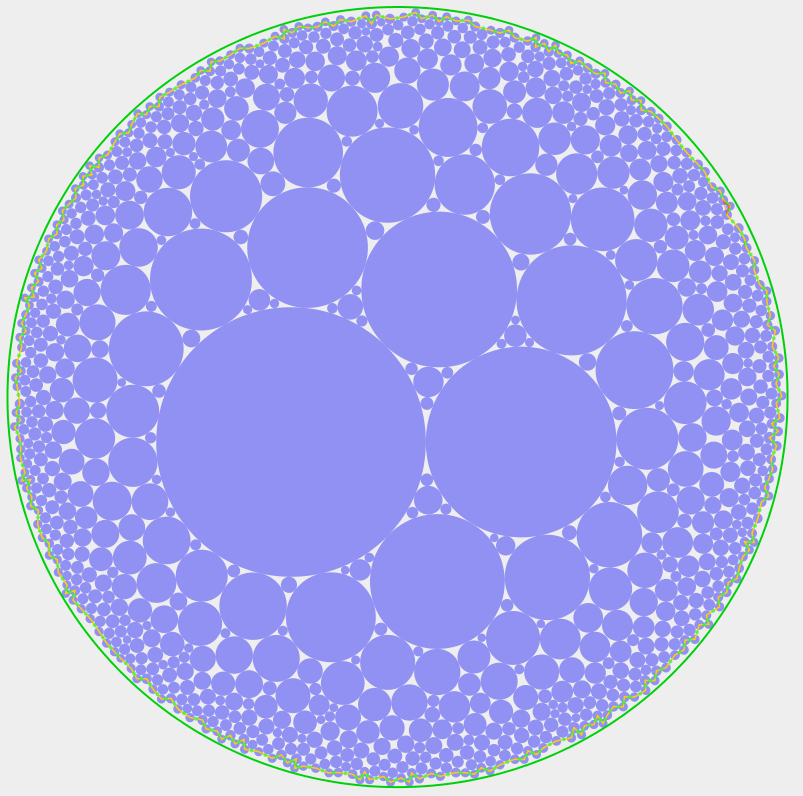
\includegraphics[width=0.65\textwidth]{packing-neg1div2-1000.png}
  \caption{Packing voor 1000 cirkels met verdeling $r_i=i^{-1/2}$} \label{fig:packing-neg1div2-1000} 
\end{figure}

\subsubsection{Bespreking}

Deze resultaten zijn volgens mij zeer indrukwekkend.
Resultaten voor de problemen $r_i = i$, $r_i = i^{1/2}$, $r_i = i^{-1/2}$ en $r_i = i^{-2/3}$ blijven steeds onder 10\% vergroting tegenover de best gekende.
Enkel het probleem $r_i = i^{-1/5}$ heeft enkele uitschieters tot maximum 13,45\% vergroting.
Dit laatste resultaat komt waarschijnlijk omdat $r_i = i^{-1/5}$ het probleem is waarin de cirkels het minst verschillen van grootte (zie \autoref{fig:packomania-verdelingen}).
Dit zorgt er voor dat het algoritme minder gebruik kan maken van gaten, aangezien meestal enkel de kleinere cirkels gaten zullen opvullen.
Het probleem met het meeste verschil in radii, $r_i = i^{-2/3}$, heeft dan ook de beste resultaten.
Met maximum 4,77\% vergroting en gemiddeld slechts 2,78\%.

Ook is er een duidelijke neerwaartse trend in de vergroting van de omschreven cirkel als het aantal cirkels groter wordt.
Dit komt doordat het algoritme dan meer keuzemogelijkheden heeft in elke stap.
Hierdoor zal het algoritme vaker gaten kunnen opvullen, en een dichtere shell opbouwen.
Hier zie je duidelijk de kracht van het algoritme als deze genoeg verschillende cirkels heeft om uit te kiezen.

Bovendien worden deze resultaten zeer snel bekomen.
Waar andere algoritmen uit de literatuur uren nodig hebben, vraagt mijn algoritme slechts milliseconden.

Dit zijn denk ik de meest indrukwekkende resultaten, en tonen het best de kracht van het algoritme.

\section{Grotere aantallen cirkels}

Het algoritme uit deze thesis laat ook toe om problemen met veel grotere aantallen cirkels op te lossen.
Resultaten voor cirkels tussen 1000 en 14000 cirkels kan je vinden in \autoref{append:packomania-tabellen-groter-aantal-cirkels}.
Ik heb geen andere methoden gevonden die problemen met zo'n grote aantallen cirkels kunnen oplossen.
De verkregen radii van de omschreven cirkel kan ik dus niet vergelijken.

De nodige tijd om deze problemen op te lossen blijft ook beperkt.
Problemen tot 1400 cirkels blijft onder één seconde.
Problemen tot 9000 cirkels onder 10 seconden, en 14000 cirkels vragen minden dan één minuut tijd.

Bij deze grote aantallen cirkels komen echter wel enkele problemen naar boven, zoals beschreven in \autoref{chap:bedenkingen}.
Ook was het niet mogelijk op mijn computer om problemen met meer dan 14000 cirkels op te lossen.
Bij het nakijken van de oplossing wordt een recursief algoritme gebruikt op de volledige lijst cirkels.
Dit geeft een \textit{stack-overflow} en heb ik nog niet kunnen oplossen.

Mits de resterende problemen met overlap voor sommige van deze problemen met grote aantallen cirkels, zijn dit interessante resultaten.
Zelfs voor duizenden cirkels kan het algoritme een resultaat geven in enkele seconden.
Dit is, voor zover ik weet, niet mogelijk met andere algoritmen in aanvaardbare tijd, laat staan in enkele seconden.

\section{Conclusie}

In dit hoofdstuk heb ik oplossingen verkregen door mijn algoritme vergeleken met de best gekende packings.
Ook heb ik de nodige rekentijd vergeleken met enkele andere algoritmen.

De oplossingen verkregen met mijn nieuwe constructieve heuristiek hebben een gemiddeld minder dan 6\% grotere omschreven cirkel.
Dit lijkt mij een zeer aanvaardbare vergroting van de omschreven cirkel, rekening houdend dat het algoritme deze problemen in slechts milliseconden op lost.
Zelfs de grootste problemen, bestaande uit duizenden cirkels, kunnen in slechts enkele seconden opgelost worden.
Ook is er een interessante neerwaartse trend in de vergroting van de radius van de bekomen omschreven cirkel.
Dit toont de kracht van het algoritme wanneer het meer cirkels heeft met verschillende radii om uit te kiezen.

Bovendien laat het algoritme toe om problemen met veel grotere aantallen cirkels in aanvaardbare tijd op te lossen.
Iets dat, voor zover ik zeet, geen enkel ander algoritme mogelijk maakt binnen aanvaardbare tijd, laat staan binnen enkele seconden.

\chapter{Verder werk} \label{chap:verder-werk}

In dit hoofdstuk geef ik enkele voorstellen voor verdere uitwerkingen van het algoritme.
Mogelijke verbeteringen, zowel in snelheid als kwaliteit van uitkomsten.
Dit zijn mogelijke ideeën om in de toekomst op verder te werken.

\section{Constante-tijd omschreven cirkel}

In het algoritme bij het plaatsen op de shell wordt gebruik gemaakt van de omschreven cirkel van de huidige tussen-oplossing.
Deze omschreven cirkel wordt berekend in lineaire tijd ten opzichte van het aantal cirkels op de shell.
Dit geeft dan de kleinst mogelijke omschreven cirkel van de huidige oplossing.

Het is echter mogelijk om in constante tijd een omschreven cirkel te berekenen.
Simpelweg door, telkens er een cirkel geplaatst wordt buiten de huidige omschreven cirkel, een nieuwe te berekenen die rond de oude omcirkel en deze nieuwe cirkel past.
Dit kan zeer eenvoudig in constante tijd, maar geeft niet de kleinst-mogelijke omschreven cirkel voor de packing.
Deze constante-tijd omschreven cirkel is mogelijk wel goed genoeg als benadering, en kan een grote snelheids-winst geven voor zeer grote packings.

\section{Best-Fit}

Het algoritme is gebaseerd op een \textit{best-fit} principe.
Met andere woorden in elke stap wordt de best-bassende cirkel gekozen.
Wat de best-passende cirkel is is echter moeilijk te bepalen.
In de huidige implementatie worden er daarom enkele keuzes gemaakt, gebaseerd op bestaande heuristieken en intuïtie.
Hier kunnen echter andere keuzes gemaakt worden, die mogelijk tot betere resultaten zullen leiden.

Eén zo'n alternatieve keuze is bij het plaatsen op de shell.
Nu worden de nieuwe cirkels zo dicht mogelijk bij het huidige middelpunt geplaatst.
Dit omdat de omschreven cirkel dan zo weinig mogelijk uitgebreid moet worden.
Maar wat als, wanneer we geen cirkel meer binnen de huidige omcirkel kunnen plaatsen, we de cirkel zo ver mogelijk van het middelpunt plaatsen (maar wel nog tegen twee cirkels op de shell)?
Dit zal er voor zorgen dat de omschreven cirkel veel verder uitgebreid zal worden.
Het zal er ook voor zorgen dat de omcirkel veel minder vaak uitgebreid moet worden, omdat hij in grotere stappen uitbreid.
Mogelijk geeft dit aanleiding tot betere en misschien snellere packings omdat de omschreven cirkel minder vaak herberekend moet worden.

\chapter{Conclusie} \label{chap:conclusie}

In deze thesis heb ik een nieuwe constructieve heuristiek voorgesteld.
Deze is gebaseerd op het \textit{best-fit} principe, waarbij in elke stap de beste cirkel gekozen wordt om aan de oplossing toe te voegen.
Deze keuze werd gebaseerd op twee concepten: \textit{gaten} en de \textit{shell}.
Eerst werden de gaten opgevuld, en dan cirkels geplaatst aan de buitenkant van de tussen-oplossing, op de shell.
Door enkele veronderstellingen te maken over het aantal cirkels die getest moeten worden voor overlap bij elke plaatsing, kan het algoritme zeer snel relatief goede packings genereren.
Ik heb resultaten getoond, vergeleken met de best-gekende packings voor een groot aantal cirkel-verdelingen, die aantonen dat het algoritme packings maakt die gemiddeld slechts 5\% groter zijn.
Deze packings werden gegenereerd in een fractie van de tijd die andere, state-of-the-art algoritmen nodig hebben (milliseconden tegenover uren).

Ik denk dus dat ik zeker geslaagd ben in mijn opzet.
Een constructief algoritme maken dat in real-time goede packings kan maken voor het zeer moeilijke \textit{cirkel-packing} probleem.

% // TODO ALGEMEEN: Minder informele termen? Omcirkel->omschreven cirkel

% // TODO ALGEMEEN: Voeg echte definities toe, bv bij Hole echt een hoofding "Definitie" en dan het gat definieren. Ook voor shell, omcirkel.

\newpage

% Appendixes

\appendix

\chapter{Packomania Benchmark Verdelingen} \label{append:packomania-benchmark-verdelingen}

\begin{tabularx}{\textwidth}{ l c X }
\caption{Packomania Benchmark Verdelingen}
\\\toprule
Instantie & N & Radii \\
\midrule
\endhead
NR10-1 & 10 & 10, 12, 15, 20, 21, 30, 30, 30, 40, 50 \\
NR11-1 & 11 & 8.4, 11, 10, 10.5, 12, 14, 15, 20, 20, 25, 25 \\
NR12-1 & 12 & 11, 12, 13, 14, 15, 16, 17, 18, 19, 20, 21, 22 \\
NR14-1 & 14 & 11, 14, 15, 16, 17, 19, 23, 27, 31, 35, 36, 37, 38, 40 \\
NR15-1 & 15 & 3, 3, 4, 4, 4.5, 6, 7.5, 8, 9, 10, 11, 12, 13, 14, 15 \\
NR15-2 & 15 & 1, 2, 3, 4, 5, 6, 7, 8, 9, 10, 11, 12, 13, 14, 15 \\
NR16-1 & 16 & 13, 14, 15, 15, 17, 19, 23, 26, 27, 27, 32, 37, 38, 47, 57, 63 \\
NR16-2 & 16 & 21, 22, 23, 24, 25, 26, 27, 28, 29, 30, 31, 32, 33, 34, 35, 36 \\
NR17-1 & 17 & 5, 5, 5, 5, 5, 5, 5, 5, 5, 5, 10, 10, 10, 15, 15, 20, 25 \\
NR18-1 & 18 & 12, 14, 16, 23, 25, 26, 27, 28, 33, 35, 47, 49, 53, 53, 55, 60, 67, 71 \\
NR20-1 & 20 & 4, 6, 8, 10, 12, 14, 16, 18, 20, 22, 24, 26, 28, 30, 32, 34, 36, 38, 40, 42 \\
NR20-2 & 20 & 6, 8, 9, 12, 12, 15, 16, 18, 20, 21, 24, 24, 27, 28, 30, 32, 33, 36, 40, 44 \\
NR21-1 & 21 & 10, 15, 16, 17, 17, 18, 21, 22, 23, 25, 26, 31, 33, 34, 37, 37, 38, 39, 40, 42, 45 \\
NR23-1 & 23 & 14, 14, 16, 18, 18, 21, 22, 23, 26, 28, 28, 32, 34, 34, 36, 37, 39, 41, 45, 48, 49, 49, 51 \\
NR24-1 & 24 & 9, 10, 11, 13, 13, 16, 17, 17, 18, 19, 19, 20, 20, 20, 21, 22, 23, 23, 24, 25, 30, 31, 32, 82 \\
NR25-1 & 25 & 14, 17, 22, 26, 26, 27, 28, 29, 29, 30, 31, 32, 33, 34, 34, 34, 34, 35, 37, 37, 37, 47, 52, 53, 55 \\
NR26-1 & 26 & 31, 32, 33, 34, 35, 36, 37, 38, 39, 40, 41, 42, 43, 44, 45, 46, 47,48, 49, 50, 51, 52, 53, 54, 55, 56 \\
NR26-2 & 26 & 41, 42, 43, 44, 45, 46, 47, 48, 49, 50, 51, 52, 53, 54, 55, 56, 57,58, 59, 60, 61, 62, 63, 64,65, 66 \\
NR27-1 & 27 & 17, 21, 25, 26, 26, 27, 27, 28, 29, 33, 33, 34, 35, 35, 35, 37, 40, 42, 43, 44, 45, 49, 53, 55, 55, 55, 63 \\
NR30-1 & 30 & 5, 8, 10, 10, 12, 14, 15, 16, 18, 20, 20, 20, 20, 20, 22, 24, 25, 26, 30, 30, 30, 30, 35, 40,40, 45, 48, 50, 55, 60 \\
NR30-2 & 30 & 6, 8, 8, 10, 12, 13, 14, 16, 18, 18, 20, 22, 23, 24, 25, 27, 28, 29,31, 33, 33, 35, 37, 38, 39,41, 43, 43, 48, 53 \\
NR40-1 & 40 & 31, 32, 33, 34, 35, 36, 37, 38, 39, 40, 41, 42, 43, 44, 45, 46, 47,48, 49, 50, 51, 52, 53, 54,55, 56, 57, 58, 59, 60, 61, 62, 63, 64, 65, 66, 67, 68, 69, 70 \\
NR50-1 & 50 & 18, 18, 19, 19, 19, 19, 21, 21, 24, 25, 25, 30, 31, 31, 33, 33, 36,36, 40, 42, 43, 46, 46, 47,49, 49, 49, 50, 50, 54, 56, 56, 57, 57, 58, 58, 59, 59, 59, 61, 62,63, 63, 64, 65, 68, 78, 79,80, 86 \\
NR60-1 & 60 & 35, 35, 35, 36, 37, 37, 38, 38, 39, 39, 40, 41, 41 ,42, 42, 42, 42,42, 44, 44, 45, 45, 46,46,47, 48, 48, 49, 50, 50, 54, 54, 57, 57, 59, 60,60, 71, 71, 71,72, 72, 74, 74, 76, 77, 77,79, 79, 80, 82, 82, 85, 86, 89, 90, 94, 95, 96, 100 \\

IN9-1 & 9 & 10, 10, 10, 10, 4.1415, 4.1415, 4.1415, 4.1415, 4.1415 \\
IN10-1 & 10 & 50, 40, 32, 31.5, 20, 20, 20, 11, 10, 10 \\
IN10-2 & 10 & 50, 40, 30, 30, 30, 21, 20, 15, 12, 10 \\
IN11-1 & 11 & 20, 19, 18, 17, 16, 15, 14, 13, 12, 11, 10 \\
IN11-2 & 11 & 25, 25, 20, 20, 15, 14, 12, 11, 10.5, 10, 8.4 \\
IN12-1 & 12 & 100, 100, 100, 48.26, 48.26, 48.26, 23.72, 23.72, 23.72, 23.72, 23.72, 23.72 \\
IN14-1 & 14 & 40, 38, 37, 36, 35, 31, 27, 23, 19, 17, 16, 15, 14, 11 \\
IN15-1 & 15 & 15, 14, 13, 12, 11, 10, 9, 8, 7, 6, 5, 4, 3, 2, 1 \\
IN16-1 & 16 & 36, 35, 34, 33, 32, 31, 30, 29, 28, 27, 26, 25, 24, 23 ,22, 21 \\
IN17-1 & 17 & 25, 20, 15, 15, 10, 10, 10, 5, 5, 5, 5, 5, 5, 5, 5, 5, 5 \\
IN17-2 & 17 & 100, 100, 100, 100, 41.415, 41.415, 41.415, 41.415, 41.415, 20, 20, 20, 20, 20, 20, 20, 20 \\
IN25-1 & 25 & 10, 10, 10, 3.533, 3.533, 3.533, 3.533, 3.533, 3.533, 2.3, 2.3, 2.3, 1.8, 1.8, 1.8, 1.8, 1.8, 1.8, 1.547, 1.08, 1.08, 1.08, 1.08, 1.08, 1.08 \\
IN28-1 & 28 & 10, 10, 10, 4.826, 4.826, 4.826, 2.371, 2.371, 2.371, 2.371, 2.371, 2.371, 1.547, 1.345, 1.345, 1.345, 1.345, 1.345, 1.345, 1.161, 1.161, 1.161, 0.9, 0.9, 0.9, 0.9, 0.9, 0.9  \\
IN162-1 & 162 & 1.8, 1.8, 1.8, 1.75, 1.3, 1.3, 1.3, 1.3, 1.3, 1.3, 1.3, 1.3, 1.3, 1.3, 1.3, 1.3, 1.05, 1.05, 1.05, 1.05, 1.05, 1.05, 1.05, 1.05, 1.05, 0.9, 0.9, 0.9, 0.9, 0.9, 0.9, 0.9, 0.9, 0.9, 0.9, 0.9, 0.9, 0.9, 0.9, 0.9, 0.8, 0.8, 0.8, 0.8, 0.8, 0.8, 0.8, 0.8, 0.8, 0.8, 0.8, 0.8, 0.8, 0.8, 0.8, 0.8, 0.8, 0.8, 0.8, 0.8, 0.8, 0.8, 0.8, 0.8, 0.8, 0.8, 0.8, 0.8, 0.8, 0.8, 0.8, 0.75, 0.7, 0.7, 0.7, 0.7, 0.7, 0.7, 0.7, 0.7, 0.7, 0.7, 0.7, 0.65, 0.65, 0.65, 0.65, 0.65, 0.65, 0.65, 0.65, 0.65, 0.65, 0.65, 0.65, 0.65, 0.65, 0.65, 0.65, 0.65, 0.65, 0.65, 0.65, 0.65, 0.65, 0.65, 0.65, 0.65, 0.65, 0.65, 0.65, 0.65, 0.65, 0.65, 0.65, 0.65, 0.65, 0.65, 0.65, 0.65, 0.65, 0.65, 0.65, 0.65, 0.65, 0.65, 0.65, 0.65, 0.65, 0.65, 0.65, 0.65, 0.65, 0.65, 0.65, 0.65, 0.65, 0.55, 0.55, 0.55, 0.55, 0.55, 0.55, 0.55, 0.55, 0.55, 0.55, 0.55, 0.55, 0.55, 0.55, 0.55, 0.55, 0.55, 0.55, 0.55, 0.55, 0.55, 0.55, 0.55, 0.55, 0.55 \\
\bottomrule
\end{tabularx}

\chapter{Packomania Vergelijking Tabellen} \label{append:packomania-tabellen}

In deze tabellen wordt telkens het aantal cirkels in de kolom $N$ gegeven, de best gekende radius van op Packomania in kolom $Beste radius$ en de radius verkregen door mijn algoritme in kolom $Radius$.
Ook wordt het absolute verschil van mijn oplossing ten opzichte van de best gekende radius in de kolom $Vergroting$ gegeven, en de procentuele vergroting in kolom $Vergroting (\%)$.
Als laatste wordt de rekentijd die mijn algoritme nodig had om tot deze oplossing te komen gegeven in kolom $Tijd$.

\section{Cirkels met gelijke grootte} \label{append:packomania-tabellen-gelijke-grootte}

Merk op dat voor het circle-packing probleem met even grote cirkels enkel de oplossingen voor $N=3$ tot $N=100$ hier getoond worden.
Dit is slechts een subset van alle gekende oplossingen.
De volledige lijst van vergelijkingen voor dit probleem, meer dan 2500 vergelijkingen, kan u terug vinden op GitHub \cite{packomania-tables-github}.

\equalTable{Packomania \ensuremath{r_i=1}}{0}{98} \label{table:packomania-equal}

\section{Packomania Macht problemen} \label{append:packomania-tabellen-macht}

\powerTable{Packomania \ensuremath{r_i=i}}{0}{196} \label{table:packomania-i}

\powerTable{Packomania \ensuremath{r_i=i^{1/2}}}{196}{292} \label{table:packomania-i^1/2}

\powerTable{Packomania \ensuremath{r_i=i^{-1/5}}}{444}{504} \label{table:packomania-i^-1/5}

\powerTable{Packomania \ensuremath{r_i=i^{-1/2}}}{292}{388} \label{table:packomania-i^-1/2}

\powerTable{Packomania \ensuremath{r_i=i^{-2/3}}}{388}{444} \label{table:packomania-i^-2/3}

Opmerking: Een oplossing voor 56 cirkels, met raddii $r_i=i^{-2/3}$ miste op de Packomania website op het moment van het schrijven van deze thesis.

\section{Packomania Benchmark problemen} \label{append:packomania-tabellen-benchmark}

\benchmarkTable{Packomania Benchmark Instances}{0}{1000}

\section{Grotere aantallen cirkels} \label{append:packomania-tabellen-groter-aantal-cirkels}

Enkel de resultaten voor meer dan 1000 cirkels wordt hier getoond.
De volledige lijst van grotere problemen, van 100 cirkels tot 14000 cirkels, kan je terug vinden op GitHub \cite{packomania-tables-github}.

\bigTable{Grotere aantallen gelijke cirkels}{130}{153}

\bigTable{Groteren aantallen cirkels: \ensuremath{r_i = i^{1/2}}}{283}{306}

\bigTable{Groteren aantallen cirkels: \ensuremath{r_i = i^{-1/2}}}{436}{459}

\bigTable{Groteren aantallen cirkels: \ensuremath{r_i = i^{-2/3}}}{589}{612}

\bigTable{Groteren aantallen cirkels: \ensuremath{r_i = i^{-1/5}}}{742}{765}

\chapter{Extra packing figuren} \label{append:extra-packing-figuren}

//TODO Update deze afbeeldingen

\section{Gelijke grootte cirkels}

\begin{figure}
  \centering
  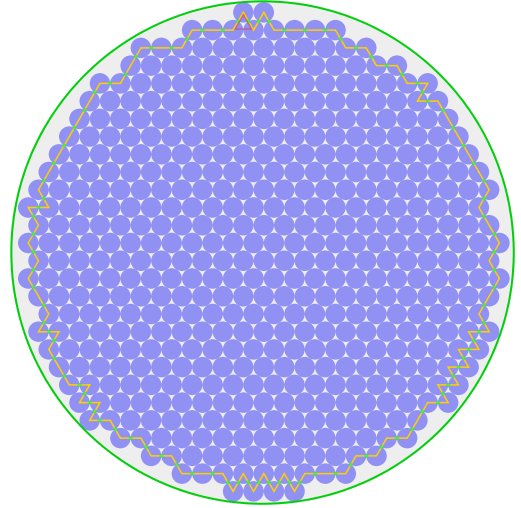
\includegraphics[width=0.65\textwidth]{packing-even-groot-500.png}
  \caption{Packing voor 500 even grote cirkels} \label{fig:packing-even-groot-500} 
\end{figure}

\begin{figure}
  \centering
  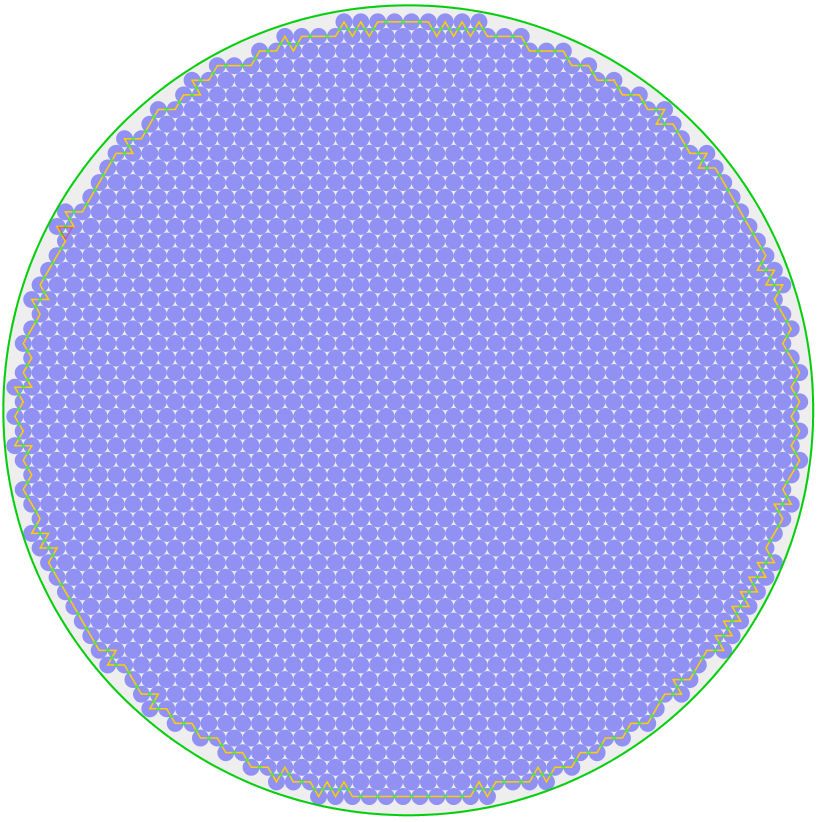
\includegraphics[width=0.65\textwidth]{packing-even-groot-2000.png}
  \caption{Packing voor 2000 even grote cirkels} \label{fig:packing-even-groot-2000} 
\end{figure}

\section{Packomania Machten}

\begin{figure}
  \centering
  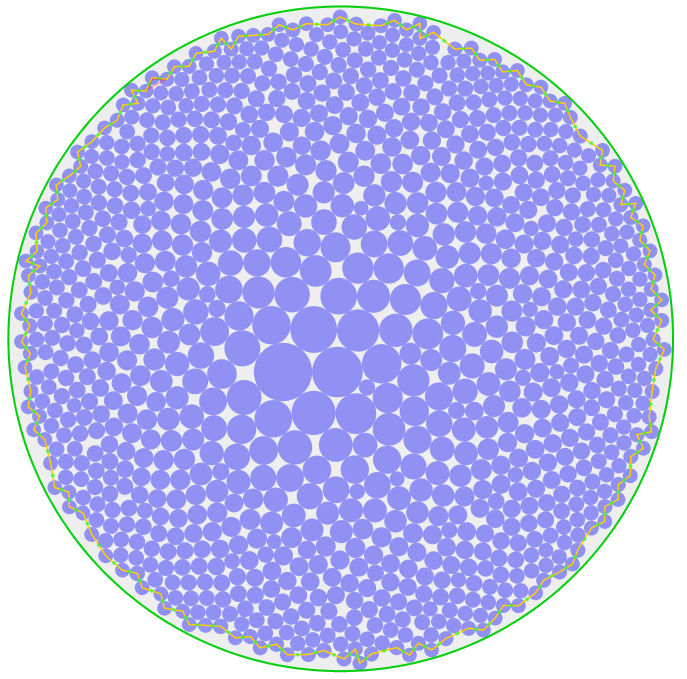
\includegraphics[width=0.65\textwidth]{packing-neg1div5-1000.png}
  \caption{Packing voor 1000 cirkels met verdeling $r_i=i^{-1/5}$} \label{fig:packing-neg1div5-1000} 
\end{figure}

//TODO: Meer afbeeldingen van machten packings

% Bibliography

\bibliography{thesis}
\bibliographystyle{plain}

\newpage

% ----------------------- Achterblad ------------------------------
% Vergeet niet de tekst aan te passen:
% - Afdeling
% - Adres van de afdeling
% - Telefoon en faxnummer
% -----------------------------------------------------------------
\thispagestyle{empty}
\sffamily
%
\begin{textblock}{191}(113,-11)
{\color{blueline}\rule{160pt}{5.5pt}}
\end{textblock}
%
\begin{textblock}{191}(168,-11)
{\color{blueline}\rule{5.5pt}{59pt}}
\end{textblock}
%
\begin{textblock}{183}(-24,-11)
\textblockcolour{}
\flushright
\fontsize{7}{7.5}\selectfont
\textbf{AFDELING}\\
Straat nr bus 0000\\
3000 LEUVEN, BELGI\"{E}\\
tel. + 32 16 00 00 00\\
fax + 32 16 00 00 00\\
www.kuleuven.be\\
\end{textblock}
%
\begin{textblock}{191}(154,-7)
\textblockcolour{}
\includegraphics*[height=16.5truemm]{sedes.png}
\end{textblock}
%
\begin{textblock}{191}(-20,235)
{\color{bluetitle}\rule{544pt}{55pt}}
\end{textblock}
\end{document}
